\documentclass{beamer}
 
% width screen 
%https://tex.stackexchange.com/questions/14336/latex-beamer-presentation-package-169-aspect-ratio
%\documentclass[aspectratio=169]{beamer}
\usepackage{comment}
\usepackage{xcolor}
\usepackage{caption}
\usepackage{graphicx}
\usepackage{array}
\usepackage{amssymb} 
\usepackage{amsmath}
\usepackage{multimedia}
\usepackage{hyperref}
\usepackage{multirow}
\usepackage{subfigure}
\usepackage{ragged2e}
\usepackage{appendixnumberbeamer}

% use speaker note
\usepackage{pgfpages}
\setbeamertemplate{note page}[plain]
\setbeameroption{hide notes} % Only slides
%\setbeameroption{show only notes} % Only notes
%\setbeameroption{show notes on second screen=right} % slides and notes
\setbeamertemplate{note page}{\pagecolor{yellow!5}\vfill\insertnote\vfill}

\renewcommand{\raggedright}{\leftskip=0pt \rightskip=0pt plus 0cm}

% beamer theme: https://hartwork.org/beamer-theme-matrix/
\usetheme{Goettingen}

% set the image paths
\graphicspath{ {imgs/} {../figures/} }
% set figure display with number
\setbeamertemplate{caption}[numbered]
\setbeamerfont{caption}{series=\normalfont,size=\fontsize{6}{8}} 

% define some colors
\definecolor{lightblue}{RGB}{0,73,114}
\definecolor{grund}{RGB}{238,241,251}          
\definecolor{schrift}{RGB}{0,73,114}
\definecolor{magenta}{RGB}{128,0,128}
\definecolor{maroon}{RGB}{113,41,21}
\definecolor{bistre}{rgb}{0.24, 0.17, 0.12} % black
\definecolor{mygrey}{rgb}{0.52, 0.52, 0.51} % grey
\colorlet{main}{green!50!black}
\colorlet{text}{bistre!100!white}

% colorized the components
\setbeamercolor{title}{fg=white}
\setbeamercolor{frametitle}{fg=white}
\setbeamercolor{section in toc}{fg=maroon}
\setbeamercolor{normal text}{fg=text}
\setbeamercolor{qed symbol}{fg=maroon}
\setbeamercolor{math text}{fg=black}
\setbeamercolor{structure}{fg=maroon, bg=maroon}
% for sidebar
\makeatletter
\setbeamertemplate{sidebar canvas \beamer@sidebarside}
[vertical shading][top=maroon!20,bottom=maroon!13]
\makeatother

% set the title box rounded and with shadow
\setbeamertemplate{title page}[default][colsep=-4bp, rounded=true, shadow=true]

% add page number of the footline
\addtobeamertemplate{navigation symbols}{}{%
    \usebeamerfont{footline}%
    \usebeamercolor[fg]{footline}%
    \hspace{1em}%
    \raisebox{1.2pt}[0pt][0pt]{\insertframenumber/\inserttotalframenumber}
}

% table of content, only display section (without subsection) with section No.
\setbeamertemplate{section in toc}[sections numbered]

% reset some component's font size in the title page
\setbeamerfont{subtitle}{size=\tiny}
\setbeamerfont{date}{size=\tiny}
\setbeamerfont{institute}{size=\tiny}

% create new command for footnote without reference
\newcommand\blfootnote[1]{%
    \begingroup
    \renewcommand\thefootnote{}\footnote{#1}%
    \addtocounter{footnote}{-1}%
    \endgroup
}
\setbeamerfont{footnote}{size=\tiny}

% ************************************************************************** %

\title[]{
	An OpenISS Framework Specialization for \\ Deep Learning-based \\Person 
	Re-identification
}
\subtitle{Master of Science Thesis Defense}
\author[]{Haotao Lai (Eric)}
%\date{\today}
\date{August 21, 2019}
\institute[] % (optional, but mostly needed)
{
	Department of Computer Science and Software Engineering\\
	Gina Cody School of Engineering and Computer Science\\
	Concordia University, Montreal, Canada
}
\titlegraphic{
\includegraphics[width=4cm]{university-logo-Concordia}}

\AtBeginSection[]{
    \begin{frame}
        \vfill
        \centering
        \begin{beamercolorbox}[sep=8pt,center,shadow=true,rounded=true]{title}
            \usebeamerfont{title}\insertsectionhead\par%
        \end{beamercolorbox}
        \vfill
    \note{\insertsectionhead}
    \end{frame}
}
% ************************************************************************** %


\begin{document}
\raggedright

\begin{frame}
\titlepage
\note{
    Thanks to Dr. Hanna for introducing me. Hello everyone, my name is Haotao 
    Lai, welcome to my master thesis defense entitled “An OpenISS Framework 
    Specialization for Deep Learning-based Person Re-identification”.
}
\end{frame}

\begin{frame}{Outline}
\tableofcontents[hideallsubsections]
\note{
    Here is the outline of my presentation, I will begin with introduction,
    then related work, followed by our solution. We will also build
    appliactions using our solution and evaluate it. At the end, conclusion
    and future work will be given.
}
\end{frame}

% ************************************************************************** %
\section{Introduction}
\subsection{Background}
\begin{frame}{Background}
	Due to our previous work \cite{iss-v2-design-theory-journal} named ISSv2, we
	were able to create artistic performance on the stage including real-time 
	motion capture, projection mapping with one Kinect v1 camera.
	\begin{figure}
		\centering
		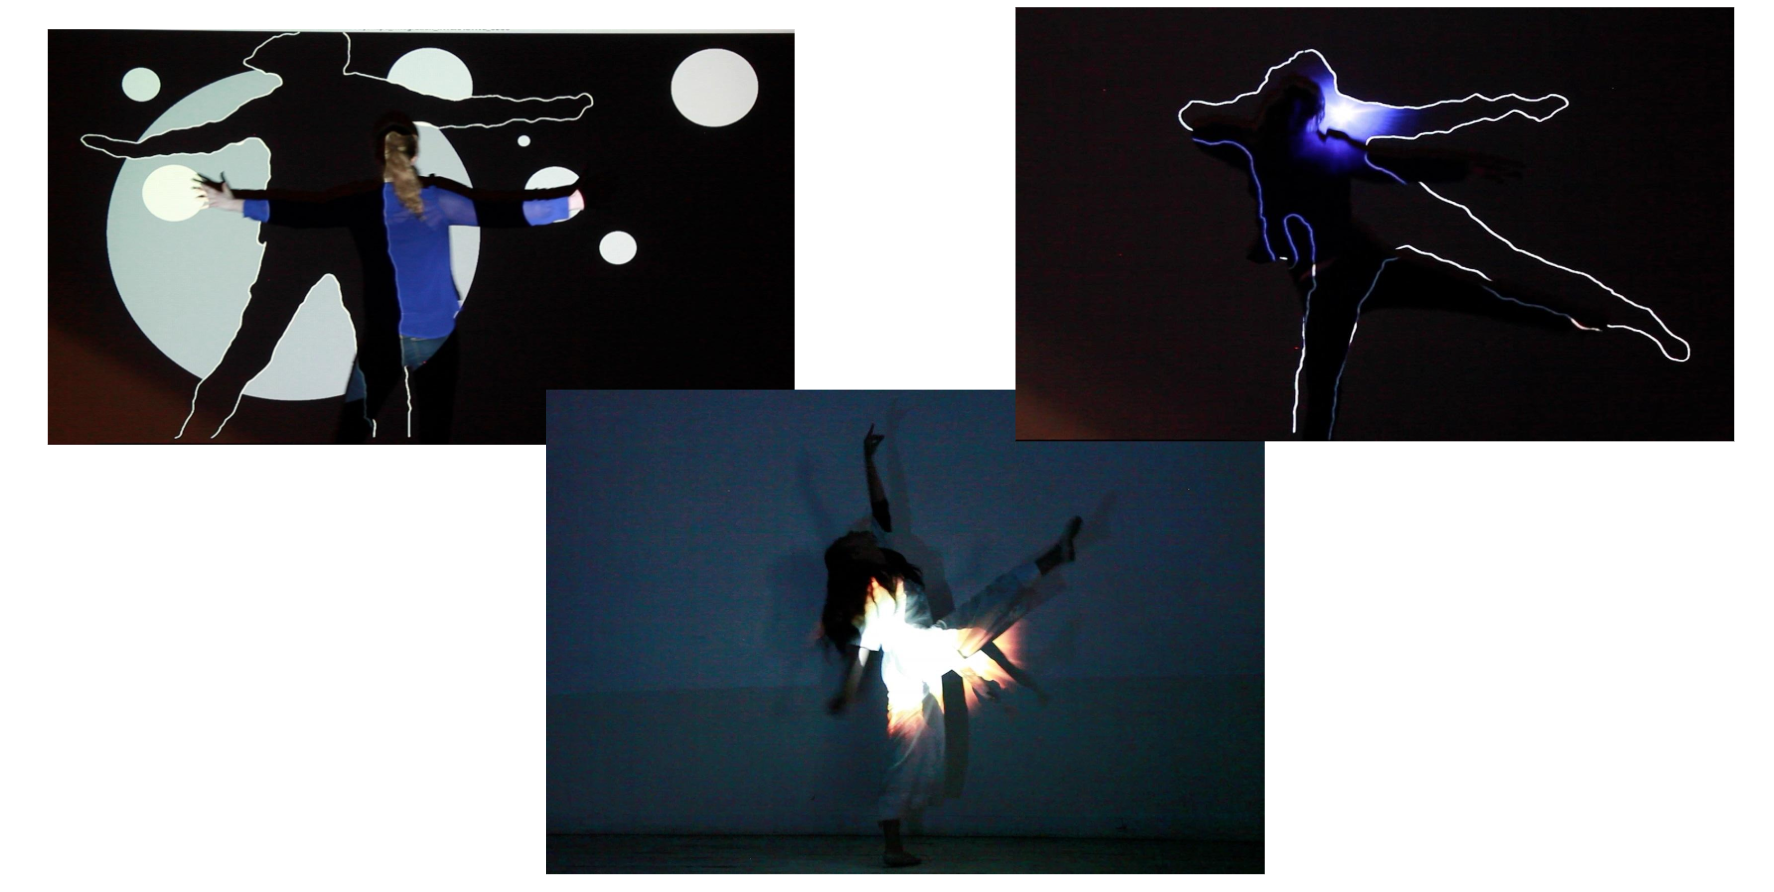
\includegraphics[width=\linewidth]{bg1.png}
		\label{fig:sub-first}
	\end{figure}

    \note{
        Due to our team’s previous work ISSv2, we were able to create 
    artistic performance including but not limited to real-time motion capture, 
    projection mapping with a single Kinect v1 camera on the stage. As you can 
    see, the two figures on top are motion capture with visual effect applied 
    and the one at the bottom is projection mapping.}
\end{frame}

\subsection{Problems}
\begin{frame}{Problems}
	When we have more chances to do our performance, we encounter the following 
	problems:
	\begin{itemize}
	    \item \textbf{PM1}: The stage is too large to cover by a single camera.
	    \item \textbf{PM2}: Various advanced cameras come to market and we 
	          would like to make our work to be compatible with them.
	\end{itemize}
	\begin{columns}
	    \begin{column}{0.6\textwidth}  %%<--- here
	        \begin{center}
	            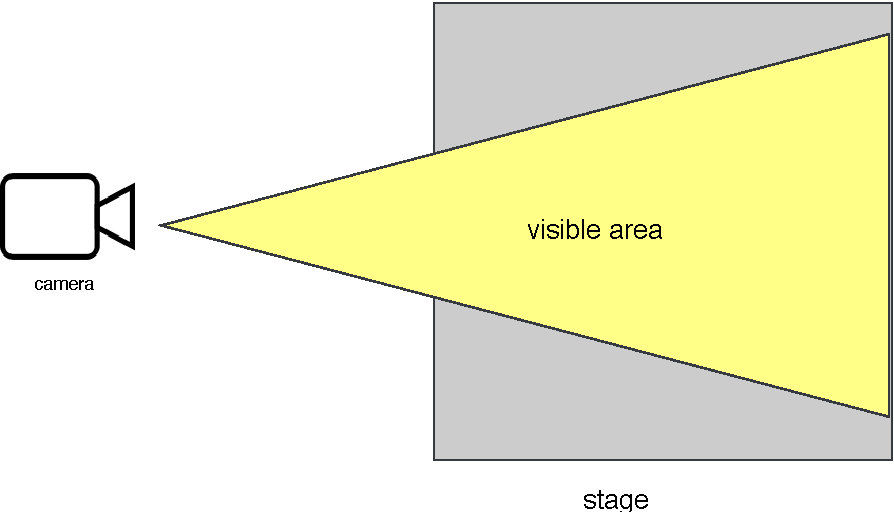
\includegraphics[scale=0.4]{probm1.pdf}
	        \end{center}
	    \end{column}
	    \begin{column}{0.4\textwidth}
		    \begin{itemize}
		        \item Kinect v1
		        \item Kinect v2
		        \item Realsense D435
		        \item ... ...
		    \end{itemize}
		\end{column}
	\end{columns}
    \note{
        But when we have more chances to do our show, we encountered two common 
        issues. One is that the stage given to us sometimes is too large and 
        cannot be covered by a single camera. And the other is that there are 
        more and more kinds of cameras with advanced features come into the 
        market but our ISSv2 can only work with Kinect v1 camera which is kind 
        of out of date now.
    }
\end{frame}

\begin{frame}{Possible Solution}
    Possible solution may be:
    \begin{itemize}
        \item For \textbf{PM1}, use more cameras to cover the stage.
        \item For \textbf{PM2}, abstract a set of common APIs for various 
              kinds of devices.
    \end{itemize}
    \begin{columns}
        \begin{column}{0.4\textwidth}  %%<--- here
            \centering
            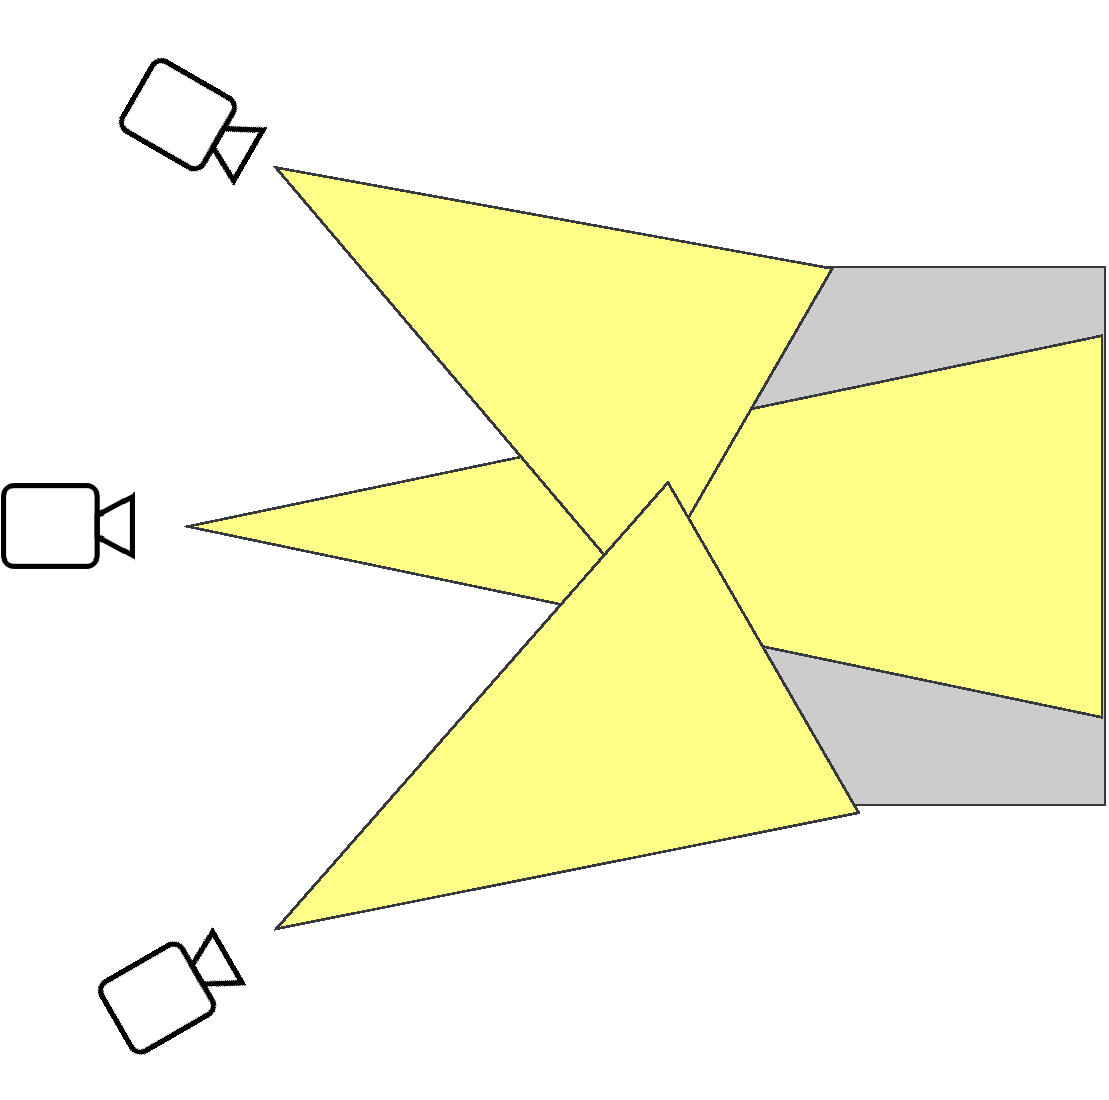
\includegraphics[width=\linewidth]{solt1.pdf}
        \end{column}
        \begin{column}{0.6\textwidth}
            \centering
            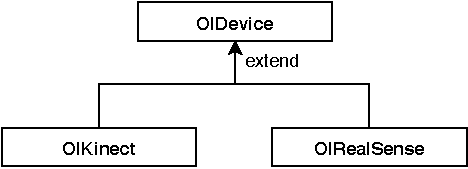
\includegraphics[width=\linewidth]{solt2.pdf}
        \end{column}
    \end{columns}
    \note{
        Natively thinking, the possible solution for problem 1 is that we can 
        use more than one camera to cover a large stage each of them will be 
        responsible for a certain area of the stage. While for problem 2 we can 
        extract the common behaviours among most of the depth cameras providing 
        an abstract layer on top of them.}
\end{frame}

\subsection{Goal}
\begin{frame}{Goal}
    To sum up, we would like to design and implement a system that with the 
    following functionalities or features: 
    \begin{itemize}
        \item device abstraction
        \item person re-identification
        \item real-time response
        \item accuracy
        \item extensibility
        \item usability
    \end{itemize}

    \note{To sum up, our solution will need to provide the following 
    functionalities or features.\\
        Device abstraction, it will be used to support various kinds of 
        cameras.\\
        Person re-identification, it is the academic term for tracking the same 
        person across multiple cameras. If we would like to cover the stage 
        with more than one camera, then we should be able to recognize the 
        actors who is whom among all the cameras we are using.\\
        Real-time response, since we are trying to solve the problem of a real 
        time show. Then our solution should be able to respond in real time.\\
        Accuracy, our solution should have a considerable accuracy since we 
        have to make sure our projection mapping and visual effect applied 
        properly.\\
        Extensibility\\
        Usability}
\end{frame}

% scenarios and requirements
\begin{comment}

\subsection{Scenarios and Requirements}
\begin{frame}{Scenarios and Requirements}{Introduction}
We have the following three usage scenarios:
\begin{itemize}
    \item device abstraction
    \item person re-identification
    \item back-end abstraction
    \item skeleton tracking
    \item interactive with other modules
\end{itemize}
\end{frame}

\begin{frame}{Scenarios and Requirements}{Introduction}
\textbf{Person Re-identification Scenario}
\begin{itemize}
    \item real-time artistic performance
    \item need to project special visual effects onto a specific actor
    \item the actor is required to have a large range of movement on the stage
\end{itemize}

\textbf{Extracted Requirements}
\begin{itemize}
    \item the process need to be done in real-time
    \item the target need to be tracked
    \item the tracking has to be done across multiple cameras
\end{itemize}
\end{frame}

\begin{frame}{Scenarios and Requirements}{Introduction}
\begin{itemize}
    {\small 
    \item \textbf{FR1}: The solution shall provide an abstraction layer 
          for the hardware that enables the physical device transparency 
          property to the users.
    \item \textbf{FR2}: The solution shall ensure the extensibility of the
          abstraction layer required in \textbf{FR1} which means when the new 
          devices come only a few or no modification need to be made and will 
          not affect the existing system.
    \item \textbf{FR3}: The solution shall be able to serve as a back-end of the
          existing ISS system providing a set of commonly used data structures 
          and functionalities for reusability.
    \item \textbf{FR4}: The solution shall be able to detect all the appearance 
          of human bodies and provide their location by bounding boxes.
    \item \textbf{FR5}: The solution shall be able to recognize a cropped image 
          with an identity cross multiple cameras if the identity has been 
          defined in advance.
    \item \textbf{FR6}: The solution shall provide the functionality to enable
          users to perform skeleton tracking among various kinds of cameras.
    \item \textbf{FR7}: The solution shall provide fundamental infrastructure
          for other modules to use and vice verse, it shall have a way to
          communicate with others voluntarily.}
\end{itemize}
\end{frame}
\end{comment}

\subsection{Contributions}

\begin{frame}{Contributions}
    \begin{enumerate}
    {\normalsize
%    {\scriptsize
        \item Design and implement a framework solution in general.\\
        {\tiny detection $|$ recognition $|$ tracking}

        \item Design and implement a device module for depth cameras 
        encapsulation.\\
        {\tiny Kinect v1 $|$ Kinect v2 $|$ RealSense D435}
        
        \item Design and implement the tracker, detector and recognizer 
        specialized frameworks.\\
        {\tiny 
        NiTE2 $\rightarrow$ skeleton tracking
        $|$         
        YOLO v3 $\rightarrow$ person detection 
        $|$ 
        ID\&Triplet Models $\rightarrow$ person ReID}
        
        \item Design a pipeline module for filter linear execution.\\
        {\tiny Person ReID application $|$ Skeleton tracking application}
        
        \item Build commonly used computer vision applications 
        using our solution.\\
        {\tiny camera calibration $|$ image alignment $|$ green screen image}
        
        \item Design and implement an dataset abstraction layer for deep 
        learning-based person ReID task.
    }
    \end{enumerate}
\end{frame}

% ************************************************************************** %

\section{Related Work}

\begin{frame}{Overview}
    Our research problem can be divided as follows:
    \begin{itemize}
    	\item person re-identification
    	\begin{itemize}
    		\item \textbf{person detection}
    		\item person tracking (omitted)
    		\item \textbf{person retrieval}
    	\end{itemize}
    	\item device abstraction
    \end{itemize}

    \note{Academically speaking, our research problem can be divided into  two 
    parts: person re-identification and device abstraction. According to the 
    research community, person ReID can be broken down into three subtasks and 
    each of them is an independent research domain. They are, person detection, 
    person tracking, and person retrieval. In our thesis, we will omit the 
    tracking problem by performing detection on each coming frame which is 
    functionally equivalent to tracking. Device abstraction is straight forward 
    we will need an abstraction layer to block the differences of various kinds 
    of depth camera.}
\end{frame}

\begin{frame}{Object Detection and Object Retrieval}
    \begin{figure}
        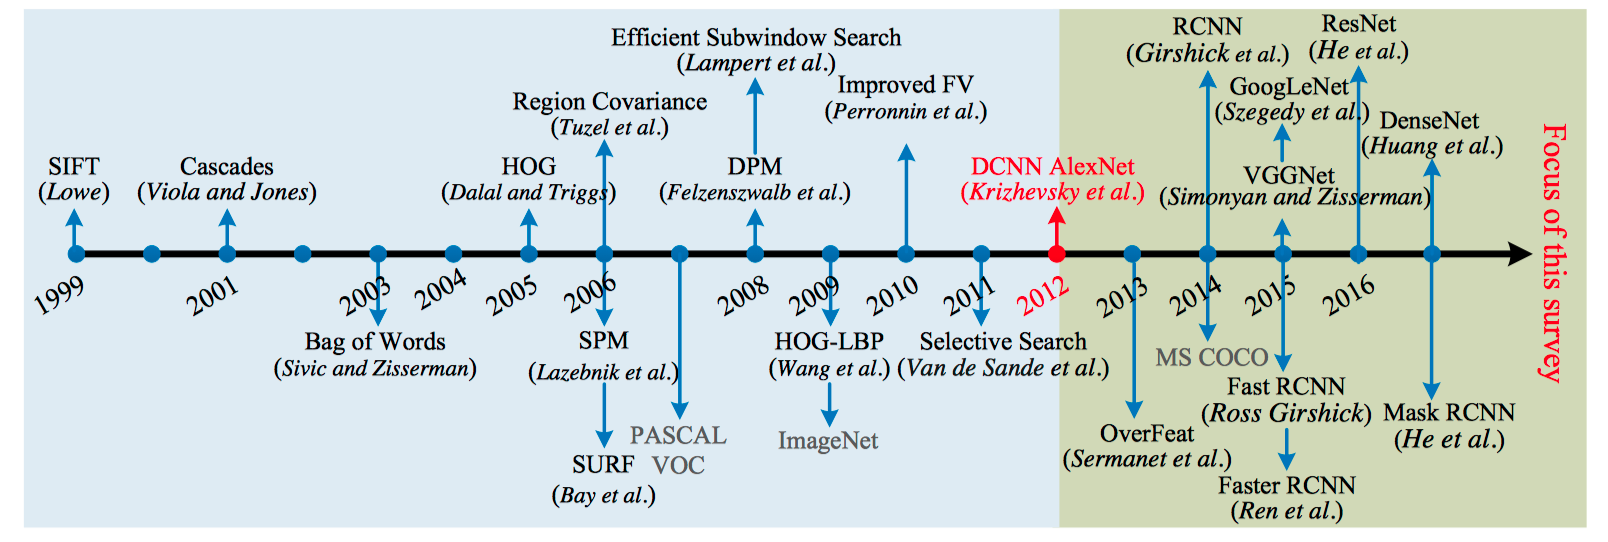
\includegraphics[scale=0.3]{timeline_od.png}
        \caption[Timeline of various methods proposed for object detection]
        {Timeline of various methods proposed for object detection
            ~\protect\cite{survey1-on-dl-od-2018}. The methods in blue area are 
            the hand-crafted detector and the methods in green area are the deep
            learning-based approaches.}
        \label{fig:od-timeline}
    \end{figure}	
    \vspace{-10px}
    \begin{figure}
        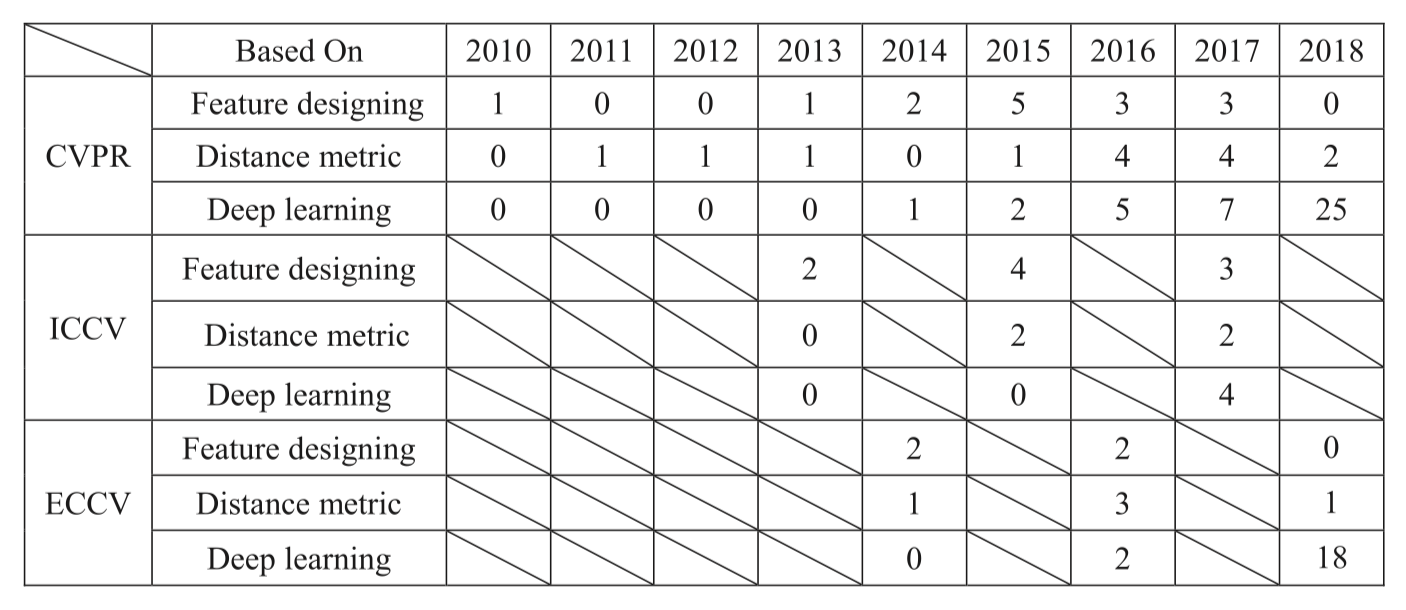
\includegraphics[scale=0.3]{papers_trend.png}
        \caption[Statistic of ReID related papers.]
        {The number of ReID papers depending on different approaches included 
            by the three top conferences in recent 
            years~\protect\cite{survey-on-dl-for-reid-2019}.}
        \label{fig:papers-trend}
    \end{figure}

    \note{Since person detection and person retrieval are subdomains of object 
    detection and object retrieval. We will first look at the research trend of 
    these two areas. In figure 1, the blue area contains hand-crafted detectors 
    while the green area contains the deep learning-based detectors , since 
    2012, the object detection research community has been dominated by the 
    deep learning-based methods. Figure 2 shows the number of paper in 
    retrieval area depending on different approaches. Since 2014, the deep 
    learning-based methods become more and more popular. So in this thesis, we 
    will only focus on the deep learning-based approach for both object 
    detection and object retrieval. We will look into these two domains 
    individually.
    }
\end{frame}

\subsection{Object Detection}
\begin{frame}{Object Detection}
    \begin{columns}
       	\begin{column}{0.5\textwidth}
       		In object detection, you are given an image $I$ and a list 
       		of classes $C$. \\
            You are asked to find all the presences of 
       		objects listed in $C$ within $I$. \\
            For each detected instance,
       		locates it using a bounding box $B$ with a confidence score $s$
            and its class label $c \in C$.
       	\end{column}
       	\begin{column}{0.4\textwidth}
            \begin{figure}
                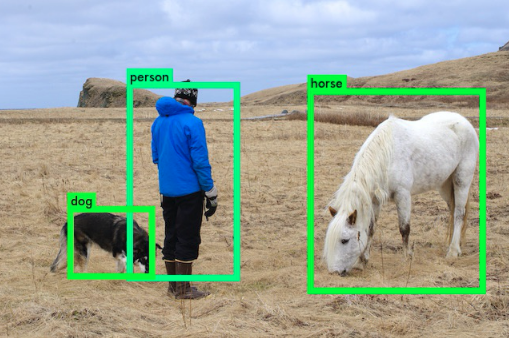
\includegraphics[width=\linewidth]{obj_det_sample_1.png}
                \caption{A sample result produced by YOLO detector.}
               	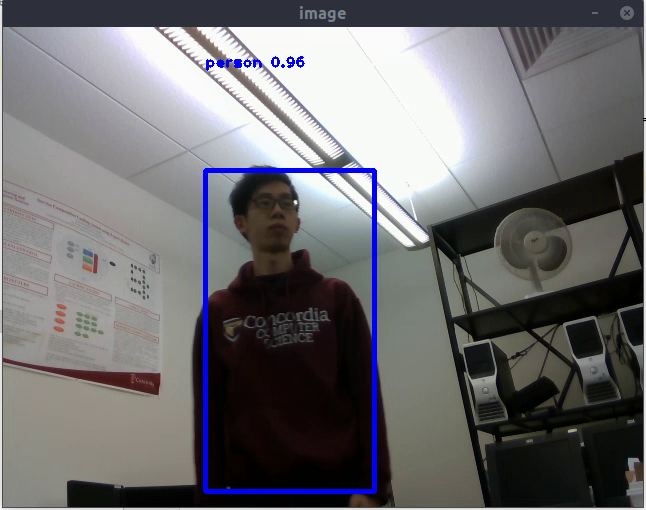
\includegraphics[width=\linewidth]{obj_det_sample_2.png}
                \caption{A sample result produced by our solution.}
            \end{figure}
       	\end{column}
    \end{columns}

    \note{The definition of object detection can be expressed as following. You 
    are given an image I and a list of classes C. You are asked to find all the 
    presences of objects listed in C within I. For each detected instance, you 
    output a bounding box, confidence score and its class label. In the right 
    handside, there are two samples output from different detectors, the one on 
    the top is from the YOLO object detector and the one below is from our 
    person detector.}
\end{frame}

\begin{frame}{Existing Solutions for Object Detection}
    \begin{itemize}
    	\item Two-stages approaches
    	\begin{itemize}
    		\item R-CNN
    		\item SPP-net
    		\item Fast R-CNN
    		\item Faster R-CNN
    		\item Mask R-CNN
    	\end{itemize}	
    	\item One-stage approaches
    	\begin{itemize}
    		\item YOLO v1
            \item YOLO v2
            \item \textbf{YOLO v3}
    		\item SSD
    	\end{itemize}
    \end{itemize}

    \note{There are already a lot of existing solutions for object detection. 
    Basically they can be categorized into two folds. One is the two-stage 
    approach and the other one is the one-stage approach. Two-stage approach 
    has an independent process for region proposal (to predict which area may 
    contain the object) while one-stage method will use regression to predict 
    the result directly. Generally speaking, the two-stage approach will slower 
    than its one-stage sibling but with a higher accuracy. In our case, we want 
    the real-time response feature since we are trying to solve the problem 
    which is part of a real-time show, we will select the one-stage method. 
    Precisely, the YOLOv3-416 approach (the 416 means the input image size is 
    416 by 416). }
\end{frame}


\begin{frame}{YOLO v3 Model Review}
    \begin{figure}
        \centering
        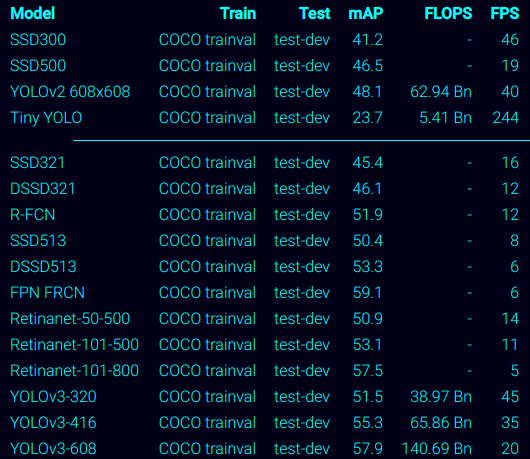
\includegraphics[scale=0.4]{yolo_vs_others_benchmark.png}
        \caption{Performance on the COCO dataset.}
    \end{figure}
    \blfootnote{
        Image is from \url{https://pjreddie.com/darknet/yolo/?source=post_page}}
    
    \note{The reason why we choose YOLOv3-416 is that it is one of the most 
    popular object detection models and there are a lot of existing resources 
    we can use directly. Also, it provides a good trade off between accuracy 
    and speed. From this figure we can see it is not the most accurate one but 
    has a good frame rate (up to 35 FpS) and only 4\% less than the most 
    accurate one.}
\end{frame}



\subsection{Person Retrieval}

\begin{frame}{Object Retrieval}
    In object retrieval, you are given a query image $p$ and a set of gallery 
    images $G$. Your task is to find the most likely image $g \in G$ for which 
    both $p$ and $g$ represent the same instance but captured by 
    different cameras.
    \vspace{10px}
    
    \begin{figure}
        \centering
        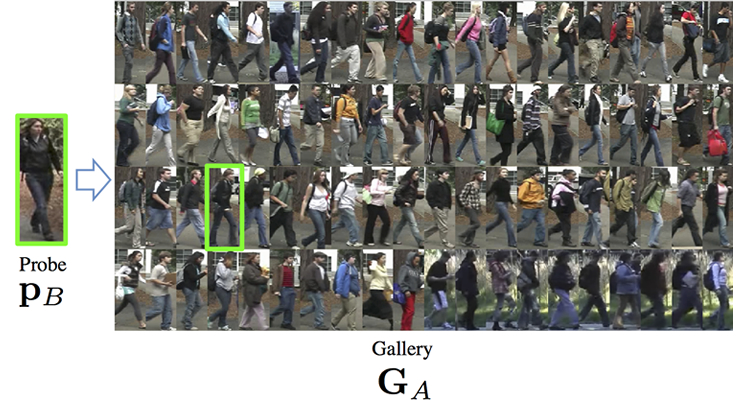
\includegraphics[scale=0.3]{reid_sample.jpg}
        \caption{An example of person retrieval process 
            \footnote{Image is from 
                \url{https://www.micc.unifi.it/projects/person-re-identification/}}.
        }
    \end{figure}    
\end{frame}

\begin{frame}{Existing Solutions for Person Retrieval}
    \begin{itemize}
    	\item \textbf{Identification model}
    	\item Verification model
    	\item \textbf{Distance metric-based model}
    	\item Parts-based model
    	\item Others
    \end{itemize}

    \note{Like the object detection, currently, the person retrieval research 
    community is also dominated by the deep learning-based approaches. The 
    existing methods for person retrieval can be categorized into the following 
    types:
        Identification model
        Verification model
        Distance metric-based model
        Parts-based model
        Others\\
        The current state of the art result is given by parts-based model but 
        again it takes more time than the others so it is not perfectly match 
        to our needs. The verification is less of accuracy. So in this thesis, 
        we are going to combine the identification model with the triplet model 
        (which is a kind of distance metric-based model). According to the 
        literature, it can produce a result with considerable accuracy and 
        acceptable speed.
    }
\end{frame}

\begin{frame}{Identification Model Review}
    ID model: the retrieval problem $\rightarrow$ classification problem. 
    \begin{itemize}
        \item {
            For each input, try to tag it with a label.}
        \item {
            The training is guided by a cross-entropy loss function.}
        \item {
            The network is actually served as a feature extractor.}
    \end{itemize}
    \centering
    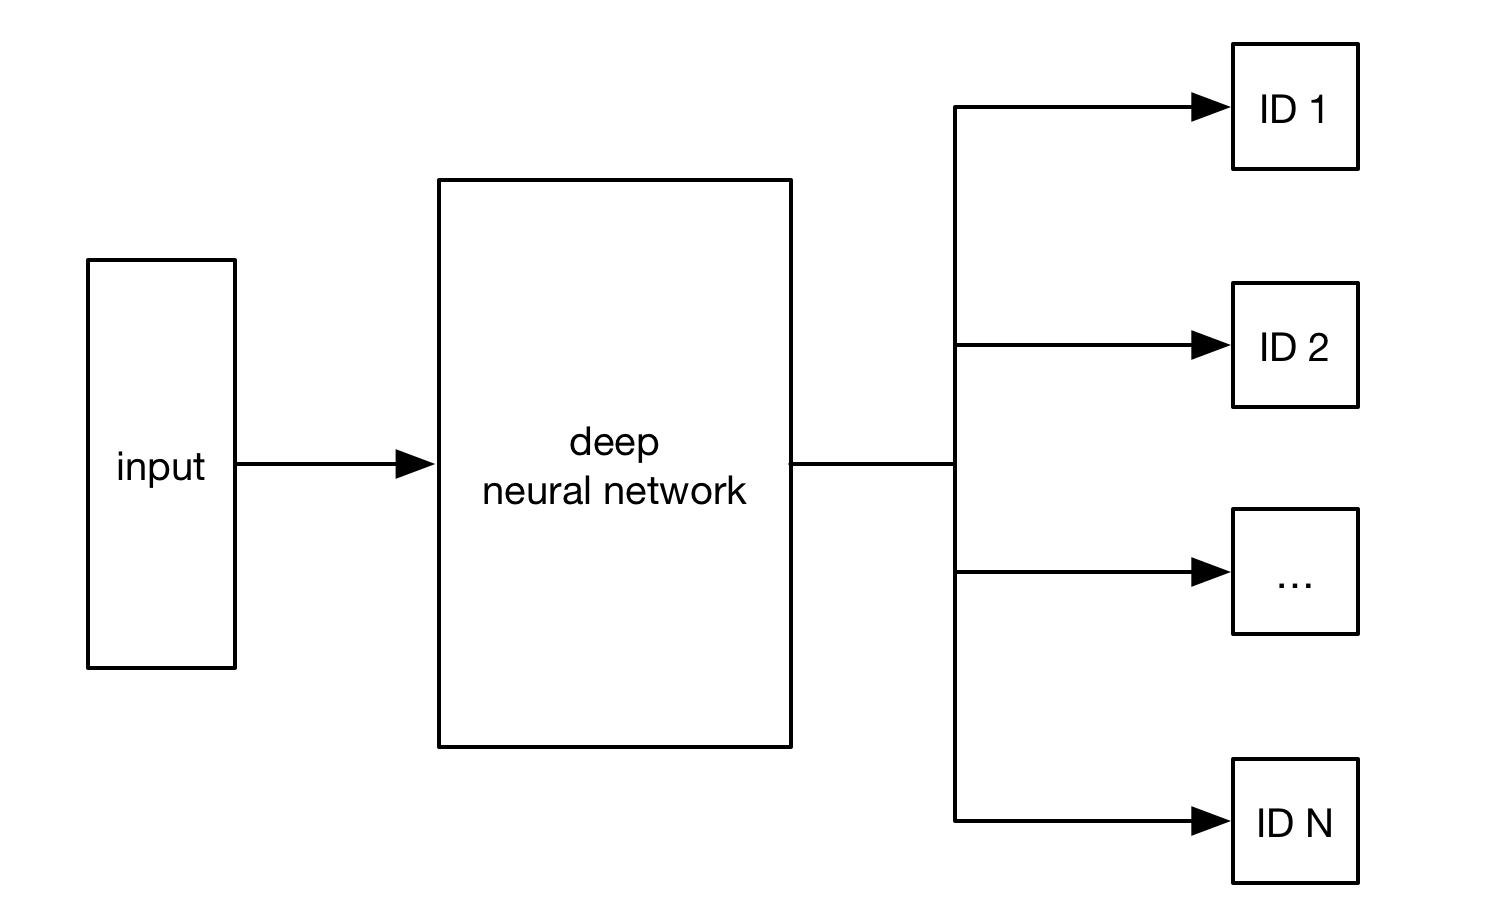
\includegraphics[scale=0.5]{id_model.png}
    
    \note{The identification model will treat the retrieval problem as a 
    classification problem. The model will try to tag each input with an id 
    label and the training is guided by the cross-entropy loss function. At the 
    end, the deep neural network will eventually become a feature extractor 
    target key features to distinguish different identities.
    }
\end{frame}

\begin{frame}{Triplet Model Review}
    \begin{columns}[T]
        \begin{column}{0.45\textwidth}
            \begin{itemize}
                \item triplet unit
                \begin{itemize}
                    \item anchor
                    \item positive
                    \item negative
                \end{itemize}
                \item distance function
                \begin{itemize}
                    \item euclidean distance
                    \item cosine similarity
                \end{itemize}
            \end{itemize}
        \end{column}
        \begin{column}{0.5\textwidth}
            \begin{itemize}
                \item loss
                \begin{itemize}
                    \item batch-all loss
                    \item batch-hard loss
                \end{itemize}
            \end{itemize}
        \end{column}
    \end{columns}

    \begin{figure}
        \centering
        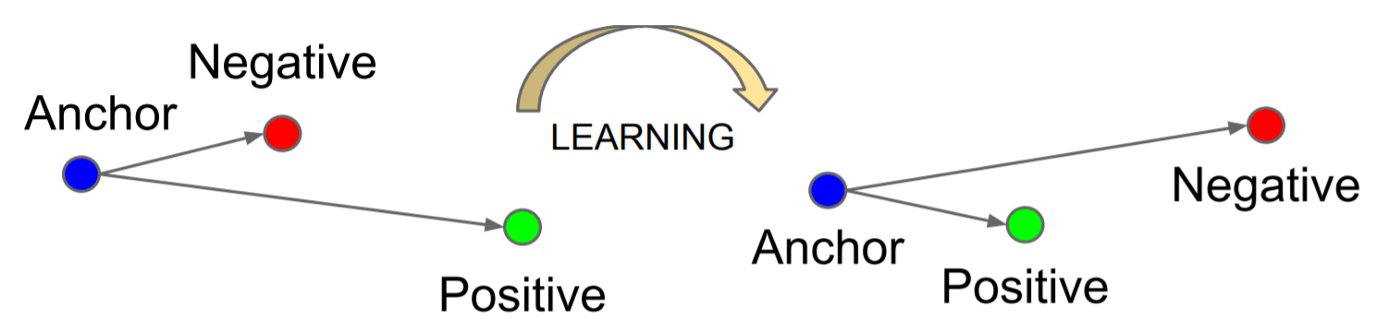
\includegraphics[scale=0.2]{triplet_objective.png}
        \caption{The learning objective of the triplet model
            ~\protect \cite{facenet-triplet-model}.}
    \end{figure}
    
    \note{There are three important components of the triplet model. A triplet 
    unit is formed by three images: anchor image, negative image, and the 
    positive image. Negative image means the id represented by this image is 
    different from the anchor image while the positive image is the inverse. 
    The learning objective of the triplet model to pull the positive image as 
    close as to the anchor image while pushing the negative image as far away 
    as possible. The close and far here are defined by the distance function. 
    Two commonly used distance functions are cosine similarity and euclidean 
    distance. The last point is the loss function, there are two candidate loss 
    functions called batch-all loss and batch-hard loss, we will explain them 
    later when we talk about evaluation.
    }
\end{frame}


\subsection{Available Software}
\begin{frame}{Available Software}
    For device abstraction:
    \begin{itemize}
        \item Freenect and Freenect2
        \item RealSense SDK
        \item OpenNI2 and NiTE2
        \item ......
    \end{itemize}
    For image processing and visualization:
    \begin{itemize}
        \item OpenCV
        \item OpenGL
        \item ......
    \end{itemize}
    For deep learning development:
    \begin{itemize}
        \item TensorFlow + Keras
        \item Pytorch
        \item ......
    \end{itemize}

    \note{Also, for implementation purposes, we survey the available software 
    which may be useful for our solution. For device abstraction, we may use 
    Freenect, Freenect2, and RealSense SDk as hardware drivers. For image 
    processing and visualization toolkit, 
    we have OpenCV and OpenGL available. And for deep learning framework, we 
    have TensorFlow plus Keras and Pytorch as our options.
    }
\end{frame}

% ************************************************************************** %
\section{Solution}

\subsection{Why Framework ?}

\begin{frame}{Why Framework Solution ?}
    Features of a software framework perfectly fit to the needs of our 
    solution so we decide to choose the framework solution.\\
    \vspace{15px}
    What is a software framework \cite{software-framework-def}:
    \begin{itemize}
        \item frozen spot
        \item hot spot
    \end{itemize}
    \vspace{15px}
    Key features of a framework \cite{wikipedia-software-framework}:
    \begin{itemize}
        \item inversion of control
        \item non-modifiable framework code
        \item extensibility
    \end{itemize}

    \note{We found that the framework’s features perfectly fit to our needs, so 
    we decided to implement our solution in the framework’s manner. We will 
    explain why.\\
        According to reference 10, a software framework consists of two 
        components:\\
        Frozen spots which define the overall architecture of a software system.
        Hot spots which represent those parts where the programmers can use to 
        write their own code to add specific functionalities based on their own 
        needs.\\
        Also, according to reference 1, there are three key features make a 
        framework different from  a software library.\\
        Inversion of control, in our case, the application developer may just 
        want the ReID result directly without knowing the intermediate process. 
        That can be done by the inversion of control, the user just tell what 
        they want and the framework will take over the control of the program 
        and return them the result.\\
        Non-modifiable framework code (frozen spots), that is used to control 
        the flow of the program to support the ioc feature.\\
        Extensibility, for example, we may want to support more kinds of 
        cameras which requires our solution to have a good extensibility.
    }
\end{frame}

\subsection{Framework Design}

\begin{frame}{Design Overview}
    Our framework named OpenISS consists of two parts:
    \begin{itemize}
        \item core framework
        \item specialized framework
    \end{itemize}
    \begin{figure}
        \centering
        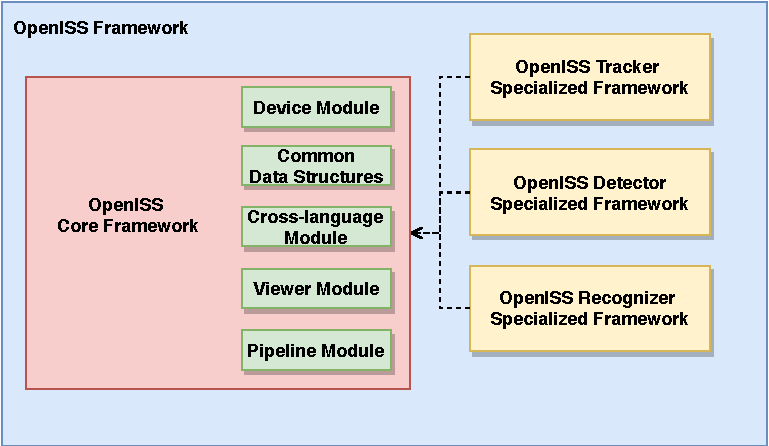
\includegraphics[scale=0.5]{framework_core_module.pdf}
        \caption{OpenISS framework architecture.}
    \end{figure}

    \note{Our proposed framework solution named OpenISS consists of two parts. 
    One is the core framework and the other is the specialized framework. The 
    core framework will provide the fundamental functionalities which may be 
    used by other core modules or specialized frameworks while each specialized 
    framework is designed to solve a specific kind of problems. We have a total 
    of five core modules for device, common data structure, cross-language, 
    viewer, and pipeline. And three specialized frameworks, they are: tracker, 
    detector, and recognizer. In the following a few slides, we will describe 
    the design of some significant modules.
    }
\end{frame}

\begin{frame}{Design of Device Module}
	\begin{columns}
		\begin{column}{0.4\textwidth}
			\begin{itemize}
				\scriptsize
				\item abstract common APIs, \\create an abstract class
				\item factory design pattern
			\end{itemize}
		\end{column}
		\begin{column}{0.6\textwidth}
			\begin{figure}
				\centering
				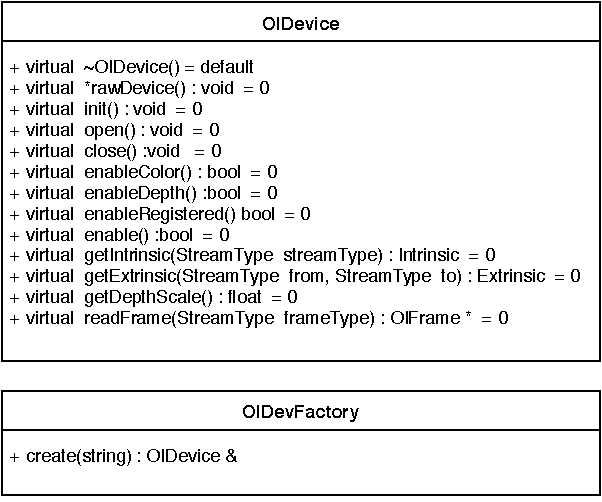
\includegraphics[width=\linewidth]{framework_core_device.pdf}
				\caption{Design of device module within OpenISS core framework.}
				\label{fig:fw-core-device}
			\end{figure}
		\end{column}
	\end{columns}
    \note{The design of the device module can be shown by this figure. We 
    abstract the methods which are common among most of the depth cameras and 
    create an abstract class named OIDevice. All the concrete device classes 
    connected to their own hardware drivers have to extend it and implement all 
    the abstract methods. Also, we employ the factory design pattern in our 
    implementation. The user will tell the factory which kind of device they 
    are expecting and the device factory will return a reference typed OIDevice 
    to hold the concrete device’s implementation.
    }
\end{frame}

\begin{frame}{Design of Cross-language Module}
    \begin{figure}
        \centering
        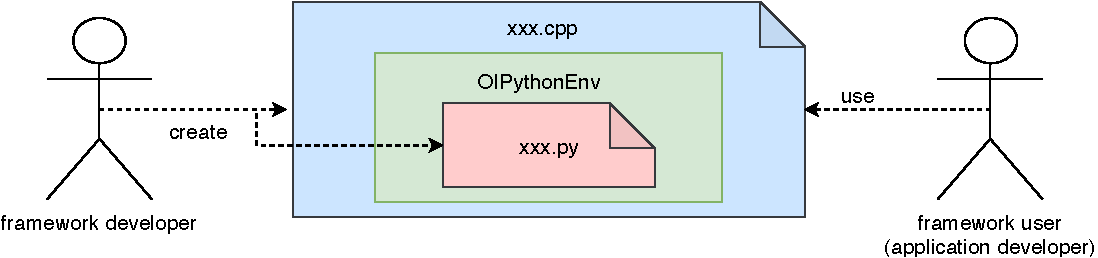
\includegraphics[width=\linewidth]{framework_core_cross_lang2.pdf}\\
    \end{figure}

    \begin{columns}
        \begin{column}{0.4\textwidth}
            \begin{itemize}
                \scriptsize
                \item most of the existing \\solutions are written in 
                \textbf{Python}
                \item our framework solution is written in \textbf{C++}
            \end{itemize}
        \end{column}
        \begin{column}{0.6\textwidth}
            \begin{figure}
                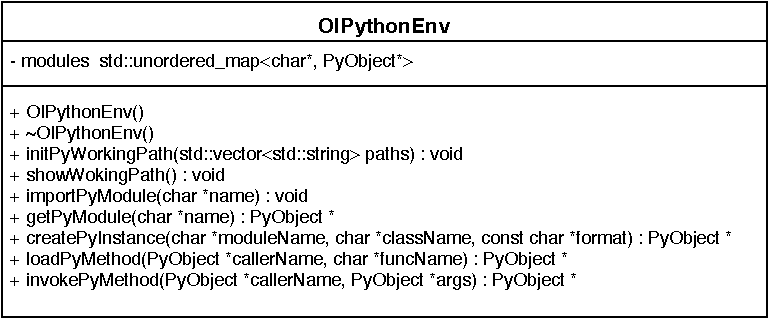
\includegraphics[width=\linewidth]{framework_core_cross_lang.pdf}
                \caption
                {Design of cross-language module within OpenISS core framework.}
            \end{figure}
        \end{column}
    \end{columns}

    \note{Then we move to the design of cross-language module. The reason why 
    we need this module is that most of the existing resources in deep learning 
    community today are written in Python. And our framework solution itself is 
    written in C++. So there is a gap between our framework and most of the 
    existing deep learning-based solutions. In order to maximize the usage of 
    the community resources, we decided to create this cross-language module 
    which can allow us to invoke Python code from C++ code as well as return 
    the result back to the callee, in our case, the C++ side. The idea is 
    simple, each instance of OIPythonEnv (shown in green) can encapsulate a 
    python script file (shown in red). The framework developer can write a 
    wrapper class (shown in blue) to hold an OIPythonEnv instance and expose 
    the target methods or variables to the framework users.
    }
\end{frame}

\begin{frame}{Design of Pipeline Module}
    \begin{figure}
        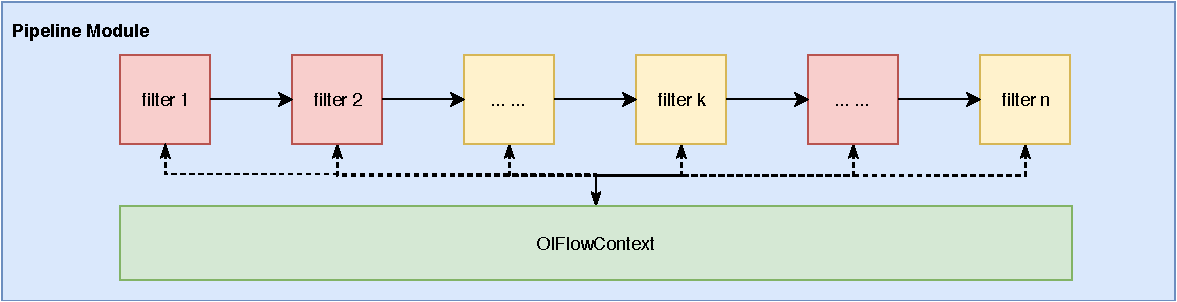
\includegraphics[width=\linewidth]{framework_core_pipeline2.pdf}
    \end{figure}
    
    \begin{columns}
        \begin{column}{0.4\textwidth}
            \begin{itemize}
                \scriptsize
                \item execution engine
                \item separate our functional modules as filters
                \item improve the reusability
            \end{itemize}
        \end{column}
        \begin{column}{0.6\textwidth}
            \begin{figure}
                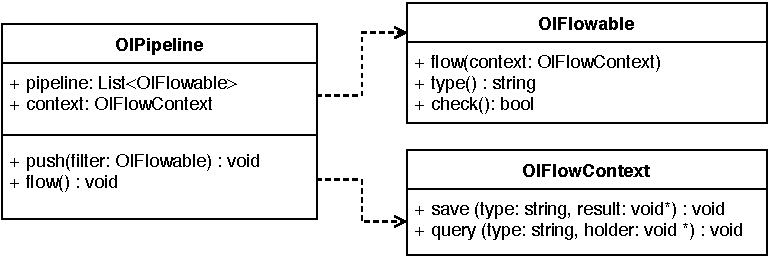
\includegraphics[width=\linewidth]{framework_core_pipeline.pdf}
                \caption
                {Design of pipeline module within OpenISS core framework.}
            \end{figure}
        \end{column}
    \end{columns}

    \note{The last module we would like to introduce in the core framework is 
    the pipeline module. It was designed as an execution engine of our 
    framework. We want to separate our functional modules as filters then a 
    working pipeline will be a chain of these filters. This filter idea can 
    improve the reusability of our framework. Within the pipeline module, we 
    have a OIPipeline class which contains a list of filter and a context 
    object. All the filters have to agree with the OIFlowable interface 
    providing implementation for flow, type and check methods. The context 
    object is a data holder of the intermediate results for all the filters.}
\end{frame}

\subsection{Framework Instantiation}

\begin{frame}{Instantiation Overview}
    \begin{figure}
        \centering
        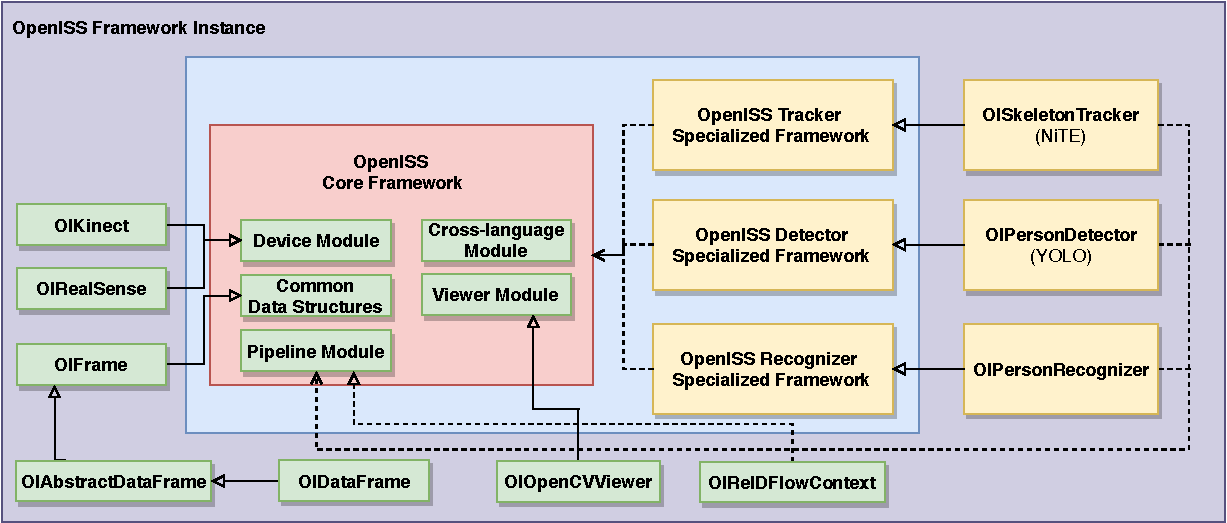
\includegraphics[scale=0.48]{framework_inst.pdf}
        \caption{OpenISS framework instance architecture.}
    \end{figure}

    \note{Then we move to the instantiation process of our framework. As you 
    can see from this figure, we create instances of the core modules shown in 
    green with purple background and three specialized framework instances 
    shown in yellow with purple background.
    }
\end{frame}

\begin{frame}{Device Module Instantiation}
    \begin{figure}
        \centering
        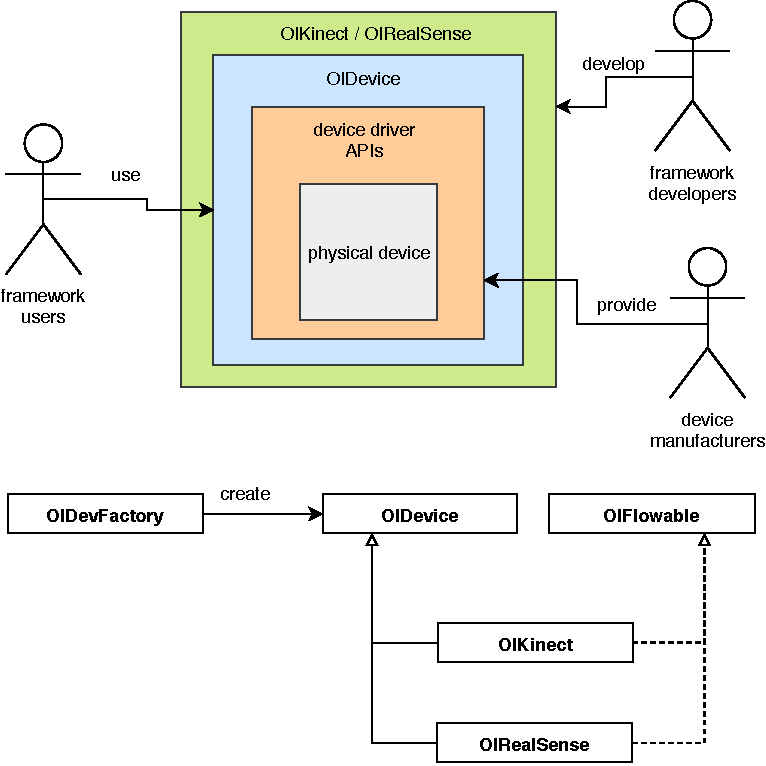
\includegraphics[scale=0.5]{device.pdf}
        \caption{Instantiation of the device module in the core framework.}
    \end{figure}

    \note{For device instantiation, as the framework developer we create two 
    concrete classes one for kinect and one for realsense cameras, both of them 
    inherit from the OIDevice class we introduced previously. Also, because of 
    the factory pattern, the framework user will only know the OIDevice. It 
    will be the device manufacturer's responsibility to provide the hardware 
    driver. Also, in order to support the pipeline module, the concrete device 
    instance agree with the OIFlowable interface.}
\end{frame}

\begin{frame}{Tracker Instantiation}
    \begin{figure}
        \centering
        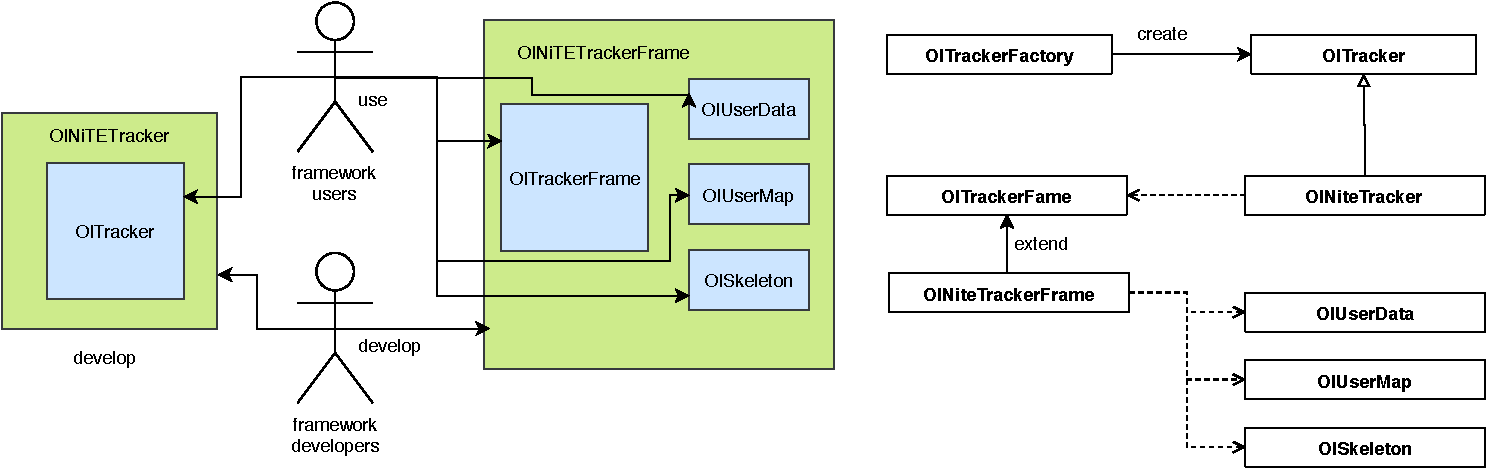
\includegraphics[scale=0.4]{framework_inst_tracker.pdf}
        \caption{Instantiation of the tracker specialized framework.}
    \end{figure}

    \note{For tracker instantiation, we don’t have our own implementation, what 
    we actually do here is porting the implementation from NiTE2 library into 
    our framework. We take the data from the NiTE2’s data structure and store 
    them back to our OpenISS common data structure then they can be consumed by 
    other components within our framework. From the implementation point of 
    view, we create OINiTETracker and OINiTETrackerFrame classes inherited the 
    OITracker and OITrackerFrame classes respectively to wrap the NiTE2’s 
    implementation and also to support the pipeline module described 
    previously.}
\end{frame}

\begin{frame}{Detector Instantiation}
    \begin{figure}
        \centering
        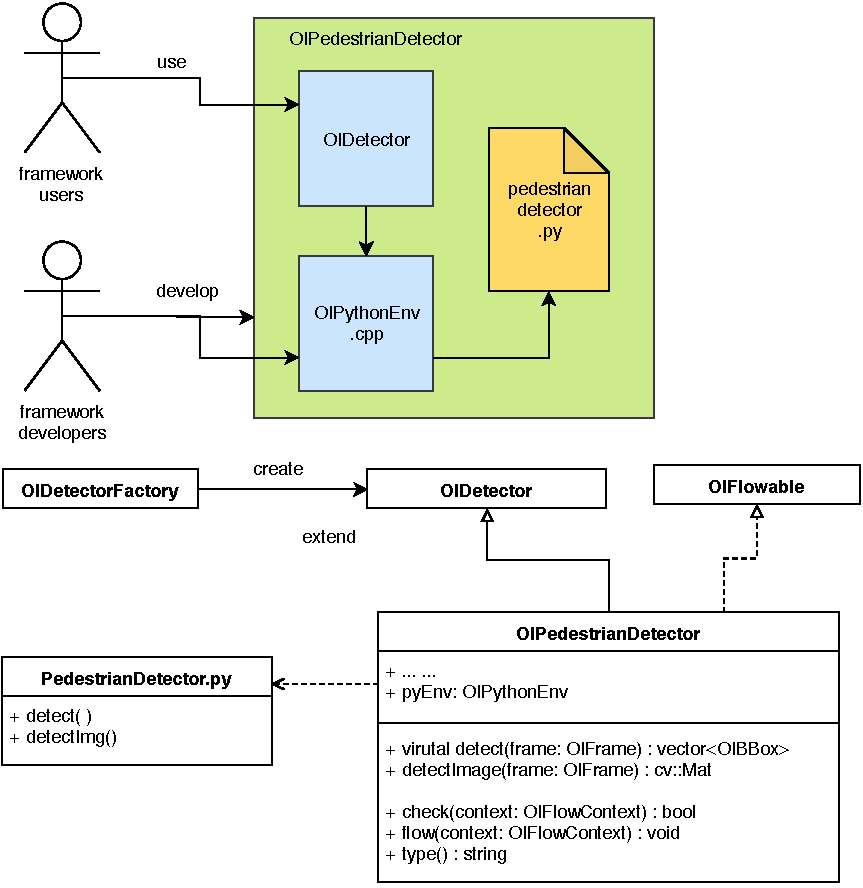
\includegraphics[scale=0.5]{framework_inst_detector.pdf}
        \caption{Instantiation of the detector specialized framework.}
    \end{figure}
    \note{For detector instantiation, we employ the YOLO v3 object detection 
    model but re-train it to become a person detector. As you can see we have 
    the persondetector.py file to hold our concrete implemented and 
    well-trained model and the OIPythonEnv to encapsulate the python script and 
    expose the necessary APIs to the framework. Then the OIPersonDetector 
    inherited from OIDetector will wrap everything up and exposed the APIs 
    defined in OIDetector to the framework user. In order to support the 
    pipeline execution workflow, OIPersonDetector also agree with the 
    OIFlowable interface.
    }
\end{frame}

\begin{frame}{Recognizer Instantiation}
    \begin{figure}
        \centering
        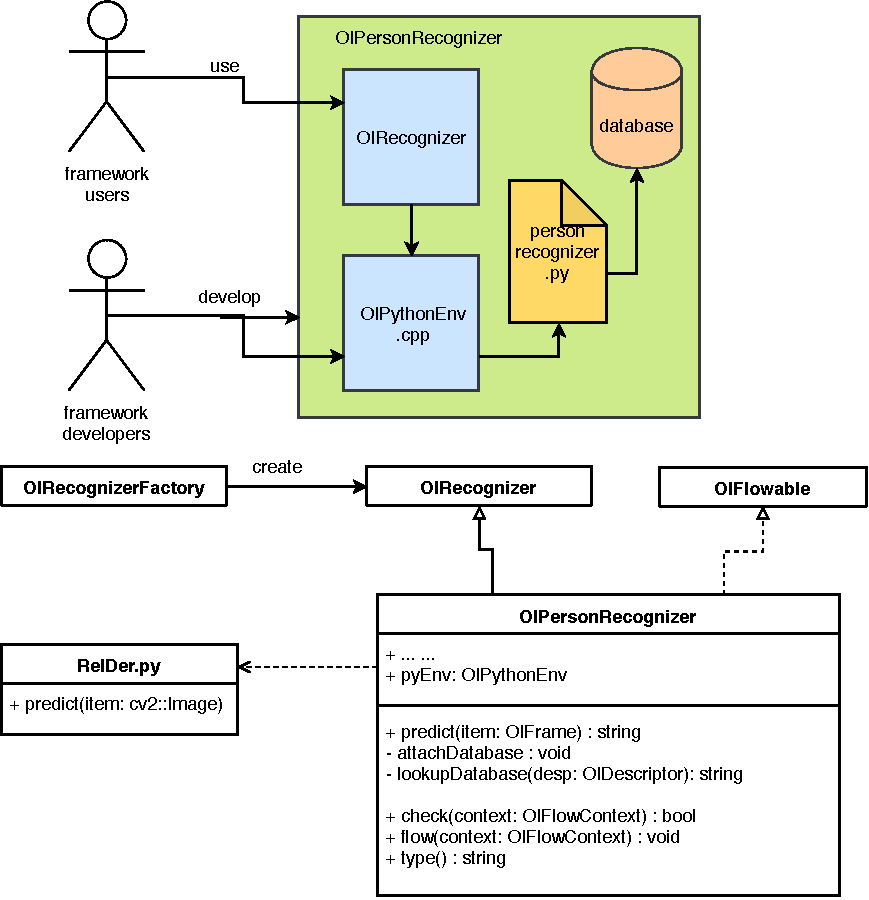
\includegraphics[scale=0.5]{framework_inst_recognizer.pdf}
        \caption{Instantiation of the recognizer specialized framework.}
        \label{fig:fw-inst-recognizer}
    \end{figure}

    \note{For recognizer instantiation, our concrete implementation is still in 
    Python so we follow almost the same structure as the detector. What’s more 
    is that for recognition problem, a database will be involved. We have the 
    methods attachDatabase and lookupDatabase to perform corresponding database 
    related operations.
    }
\end{frame}

\begin{frame}{Design and Instantiation Summary}
    Framework implementation aspect:    
    \begin{itemize}
        \item Design and instantiate 5 core modules.
        \item Design and instantiate 3 specialized frameworks.
    \end{itemize}
    \vspace{10px}
    Deep learning-based model aspect:
    \begin{itemize}
        \item Re-implement the YOLO v3 model
        and retrain it from an object detector to person detector with 
        existing training facilities 
        \footnote{https://github.com/qqwweee/keras-yolo3}.
        \item Integrate the mAP benchmark facilities
        \footnote{https://github.com/Cartucho/mAP} for YOLO model.
        \item Re-implement the recognizer model from scratch on top of 
        TensorFlow and Keras with reference 
        \footnote{https://github.com/michuanhaohao/reid-strong-baseline} in 
        Pytorch.
    \end{itemize}

    \note{Before we move to the application section, we would like to emphasize 
    our contribution. In the framework aspect, we design and instantiate 5 core 
    modules and 3 specialized frameworks.\\
        In the deep learning model aspect\\
        We re-implement the YOLO v3 model and retrain it from an object 
        detector to person detector with existing training facilities.\\
        We integrate the mAP benchmark facilities for YOLO model.\\
        We re-implement the recognizer model from scratch on top of 
        TensorFlow and Keras with reference in Pytorch.

    }
\end{frame}

% ************************************************************************** %
\section{Applications}

\begin{frame}{Overview}
    \begin{figure}
        \centering
        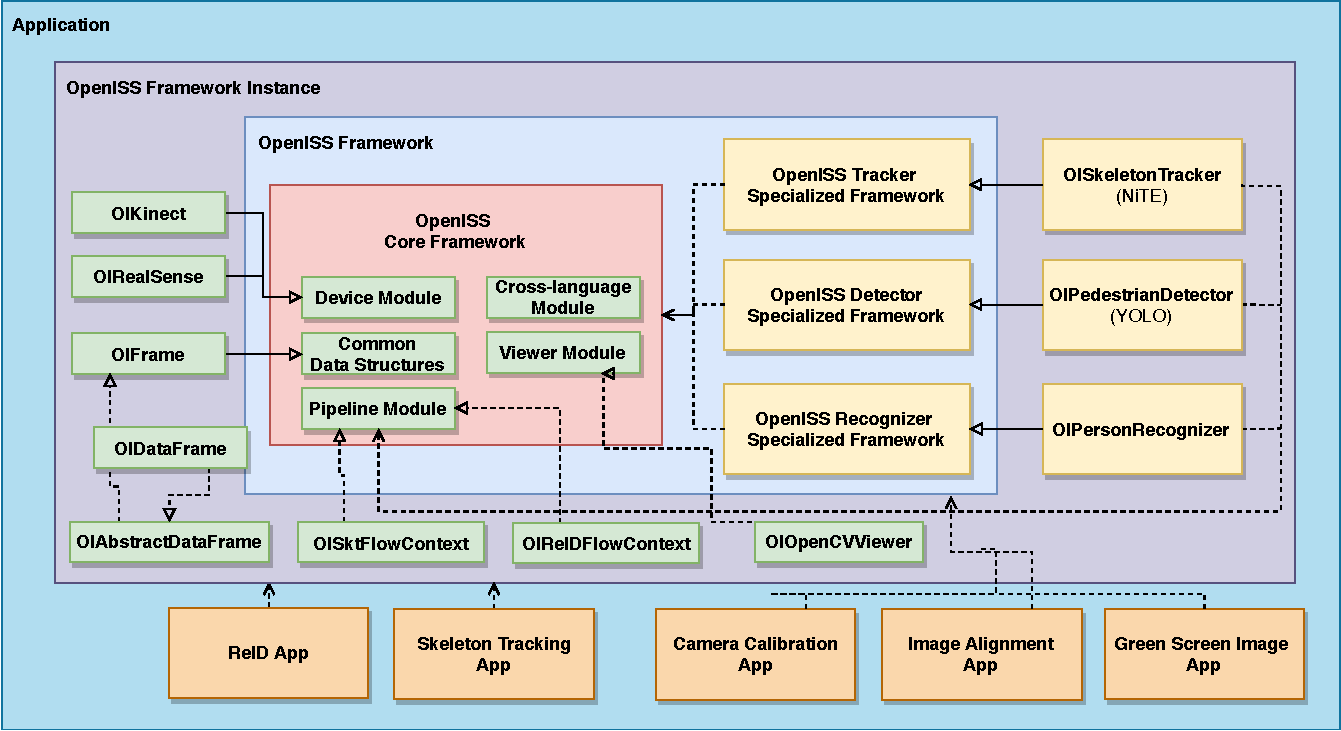
\includegraphics[scale=0.45]{framework_app.pdf}
        \caption{OpenISS framework instance architecture with applications.}
    \end{figure}

    \note{From this figure, we can see, currently we have five applications, 
    shown in orange with blue background. They are:\\
        Person re-identification application\\
        Skeleton tracking application\\
        Camera calibration application\\
        Image alignment application\\
        Green screen image application\\
    }
\end{frame}

\subsection{Person ReID}

\begin{frame}{ReID Application}
    \begin{figure}
        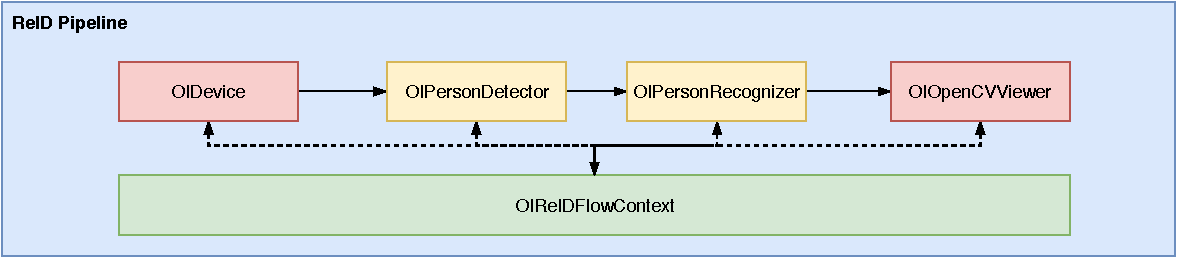
\includegraphics[width=\linewidth]{framework_app_reid_pipeline.pdf}
        \caption{Skeleton tracking pipeline.}
    \end{figure}
    \vspace{-20px}
    \begin{columns}
       \begin{column}{0.4\textwidth}
            \begin{figure}
                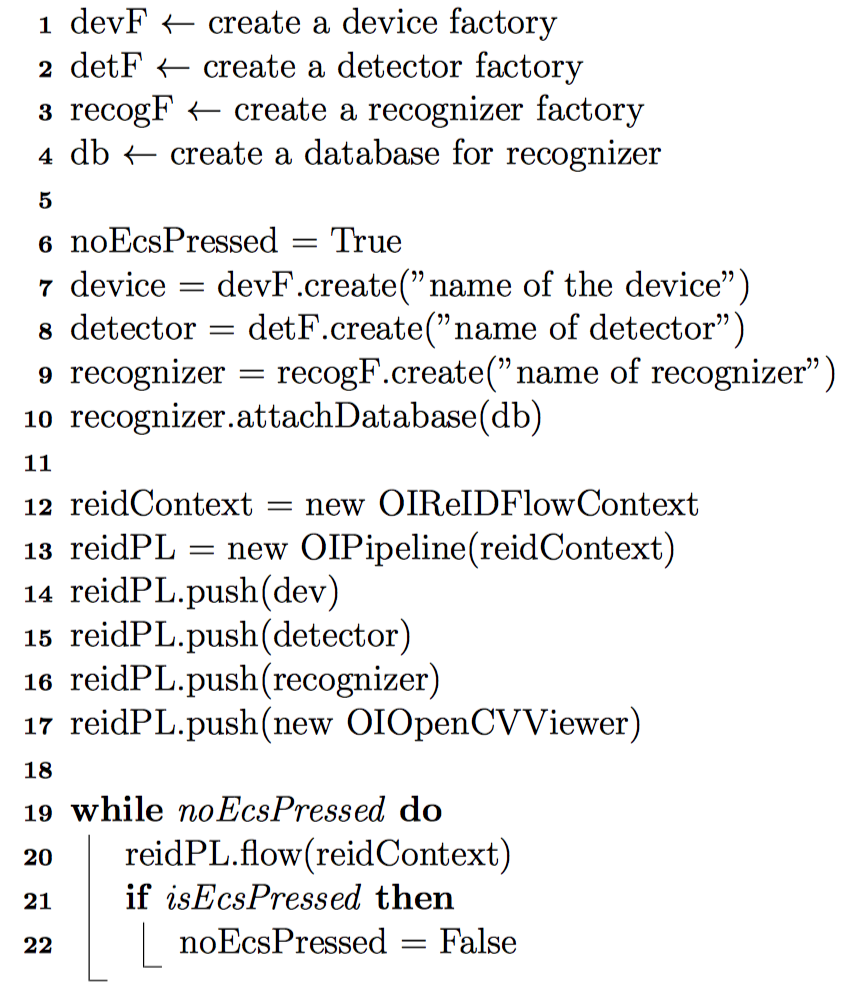
\includegraphics[width=\linewidth]{reid_algo.png}
            \end{figure}
       \end{column}
       \begin{column}{0.6\textwidth}
           \begin{figure}
               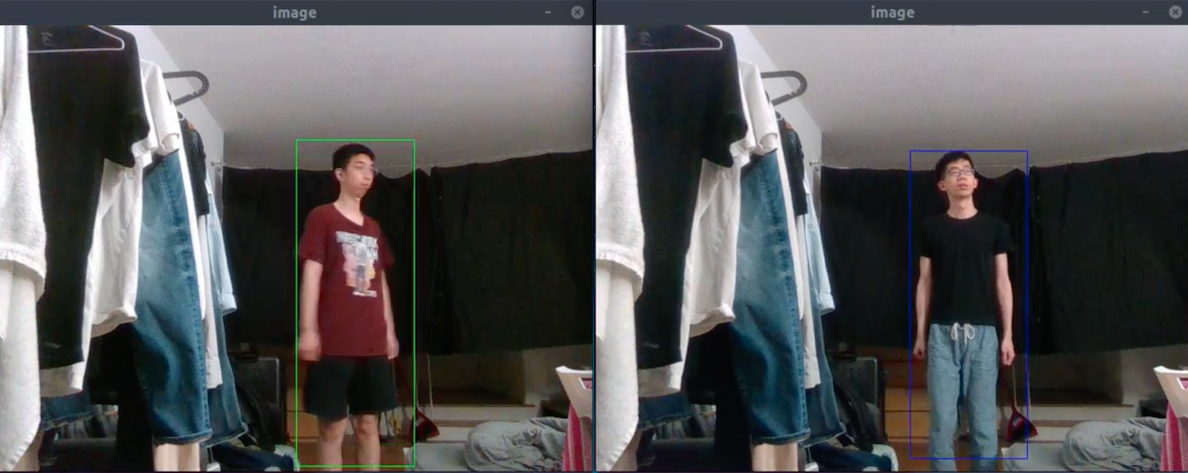
\includegraphics[width=\linewidth]{reid_result.png}
               \caption{Person ReID application.}
           \end{figure}
       \end{column}
    \end{columns}

    \note{First, we introduce the ReID application. The logic of this 
    application can be demonstrated by the pseudocode shown on the 
    left-hand-side. We create factory instances for device, detector, and 
    recognizer respectively. Then we create the filter instances using the 
    corresponding factory. Finally we push all these filter instances into the 
    pipeline and invoke the pipeline.flow method. After the pipeline 
    construction is done, the ReID pipeline will look like the figure shown on 
    top of the slide. In this specific application, we pre-record a database 
    contains two identities in advance using a camera which is different from 
    the one we use during the experiment. The result of this application can be 
    shown by the figure at the bottom of right-hand-side, identity1 is 
    recognized and a green bounding box is drawn around him. And for identity2, 
    a  bounding box in another colour, blue, is drawn.
    }
\end{frame}

\subsection{Skeleton Tracking}

\begin{frame}{Skeleton Tracking Application}
    \begin{figure}
        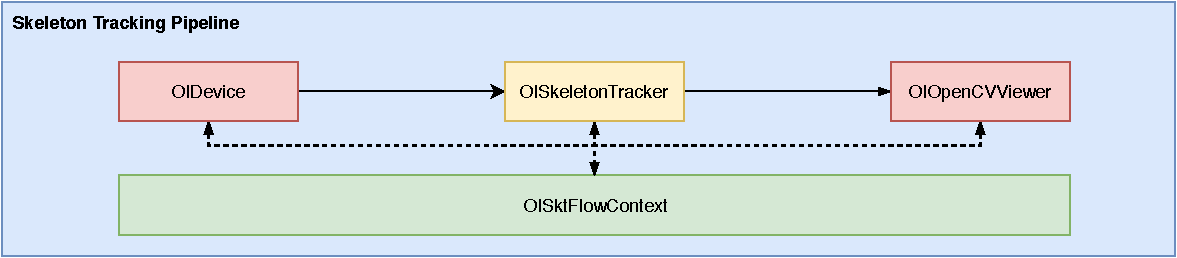
\includegraphics[width=\linewidth]{framework_app_skt_pipeline.pdf}
        \caption{Skeleton tracking pipeline.}
    \end{figure}    
    \vspace{-20px}
    \begin{columns}
        \begin{column}{0.4\textwidth}
            \begin{figure}
                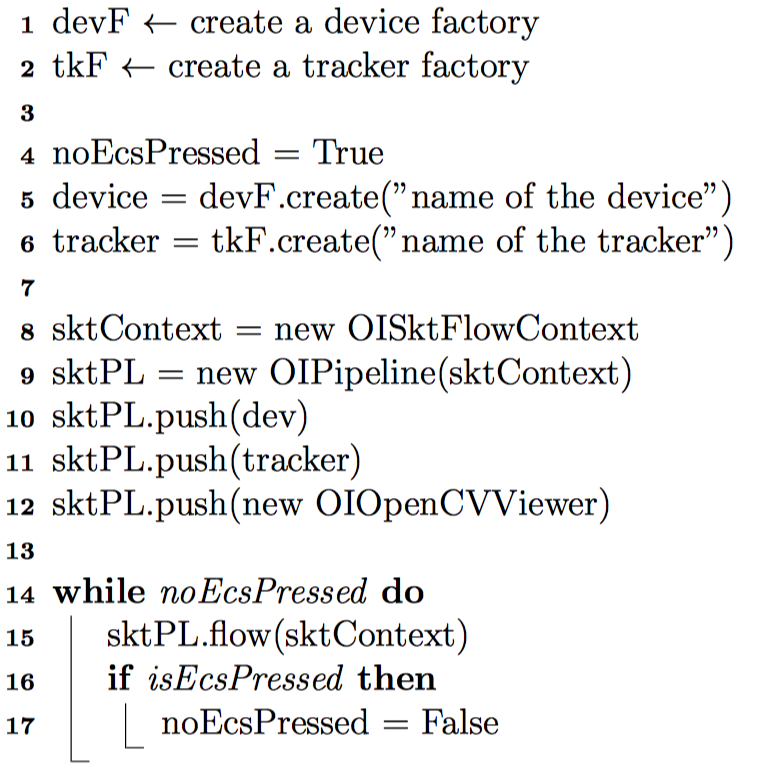
\includegraphics[width=\linewidth]{skt_algo.png}
            \end{figure}
        \end{column}
        \begin{column}{0.6\textwidth}
            \begin{figure}
                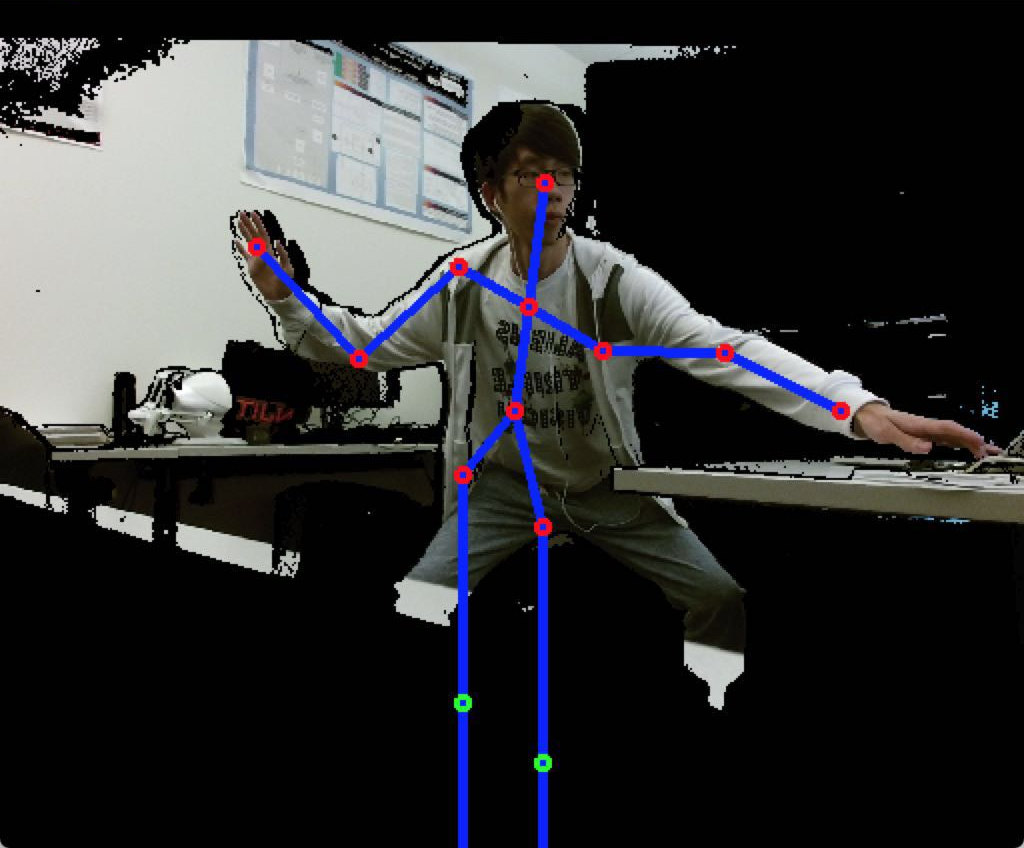
\includegraphics[scale=0.1]{framework_skeleton.png}
                \caption{Skeleton tracking application.}
            \end{figure}
        \end{column}
    \end{columns}

    \note{Follow the same pattern, we have the skeleton tracking application. 
    As you can see from the result image, the skeleton of the detected person 
    has been extracted, we use a total of 13 points to describe a person’s 
    skeleton. That may be useful when we do project mapping or apply special 
    visual effect on a certain place of a human body.}
\end{frame}

\subsection{Others}

\begin{frame}{Other Applications}
     \begin{columns}
        \begin{column}{0.5\textwidth}
           Other applications:
           \begin{itemize}
               \item camera calibration
               \item image alignment
               \item green screen image
           \end{itemize}
        \end{column}
        \begin{column}{0.4\textwidth}
            \begin{figure}
                 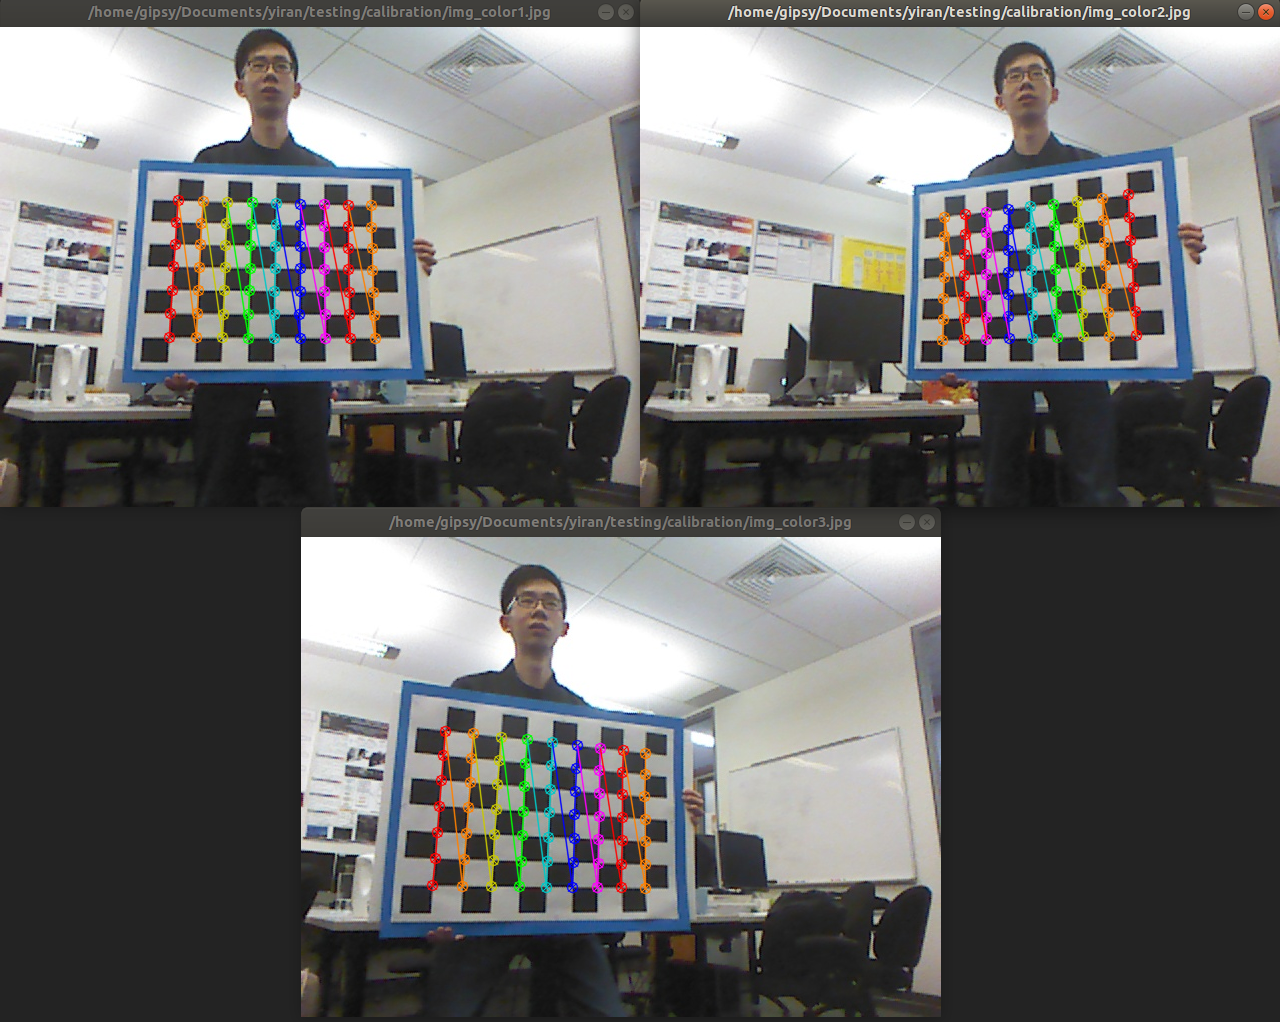
\includegraphics[width=\linewidth]{framework_app_calib.png}
                 \caption{Camera calibration application.}
            \end{figure}
            \begin{figure}
                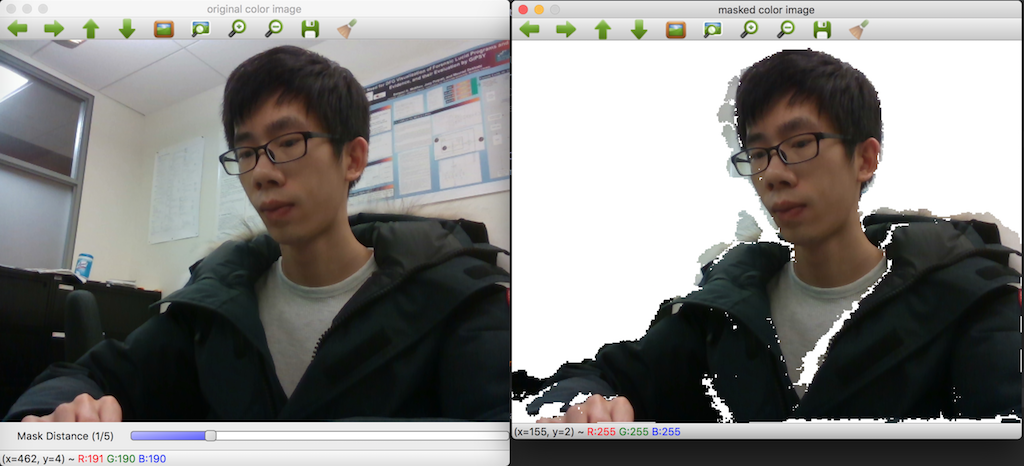
\includegraphics[width=\linewidth]{framework_greenscreen.png}
                \caption{Green screen image application.}
            \end{figure}
        \end{column}
    \end{columns}
    \note{We have three more other applications, figure is the sample result 
    from camera calibration and figure is the sample result from green screen 
    image.}
\end{frame}

% ************************************************************************** %
\section{Evaluation}
\subsection{Framework Evaluation}
    
\begin{frame}{Framework Evaluation}
     \begin{itemize}
        \item Functional Requirements
        
            \begin{itemize}
                \item person re-identification
                \item skeleton tracking
                \item device abstraction
            \end{itemize}
        
        \item Non-functional Requirements
        
            \begin{itemize}
                \item real-time response
                \begin{itemize}
                    \item higher than 10 FPS, human perceive them as motion
                    \cite{wikipedia-frame-rate}
                    \item our solution achieve 12 FPS (acceptable)
                \end{itemize}
                \item accuracy
                \begin{itemize}
                    \item ranked 9th/32 on Market1501 dataset
                    \item ranked 7th/27 on DukeMTMC-reid dataset
                \end{itemize}
                \item extensibility
                \begin{itemize}
                    \item device module
                    \item tracker specialized framework
                \end{itemize}
                \item usability
                \begin{itemize}
                    \item 1 line of application code change for switching device
                    \item 36 lines of application code to enable person ReID 
                    feature
                \end{itemize}
            \end{itemize}
    \end{itemize}
%    \note{In the evaluation section, we are going to evaluate our solution 
%from 
%    two aspects. One is the framework evaluation which will demonstrate our 
%    framework solution can actually fulfill both the functional and 
%    non-functional requirements. And the other is algorithm/model evaluation 
%    which can tell how well our solution can achieve compared to the 
%    state-of-the-art result.
%    }

    \note{
        We will first evaluate the our solution based on the requirements. As 
        for the functional requirement, the applications we introduced 
        previously have proved we can achieve them.
        Let's take a look to the non-functional requirements.\\
        In term of real-time response, our solution achieve 12 FPS while a
        just-display application is 20 FPS. According to reference 1, if the
        frame rate is higher than 10 FPS, human will perceive it as motion.
        So we solution is acceptable in the context of speed.\\
        Our solution can also provide a considerable accuracy compared to the
        state of the art result, we will discuss it later.\\
        Device module and tracker specialized framework are good showcases to
        prove that our solution comes with a good extensibility.\\
        And for usability, we only need to change 1 line of code to switch 
        device and only 36 lines of code to enable a complex feature, for 
        example, the ReID feature.
    }
\end{frame}

\subsection{ReID Evaluation}

\begin{frame}{Environment Setting}
    Two environment settings:
    \begin{itemize}
        \item \texttt{setting 1}: a desktop machine
        \item \texttt{setting 2}: a powerful GPU cluster
    \end{itemize}
    \begin{table}[]
        \centering
        \scalebox{0.6}{%
            \begin{tabular}{|l|l|c|l|}
                \hline
                \multicolumn{1}{|c|}{\textbf{Setting}} &
                \multicolumn{1}{c|}{\textbf{Name}} & \textbf{Amount} &
                \multicolumn{1}{c|}{\textbf{Device}} \\ \hline
                \multirow{4}{*}{1(Desktop Machine)} & Memory & 1 & 8 GB \\ 
                \cline{2-4}
                & Processor & 1 & Intel Core i5-3470 CPU @3.20GHz $\times$ 4 \\
                \cline{2-4}
                & Graphics & 1 & GeForce GTX 1070 Ti (8GB memory) \\ \cline{2-4}
                & OS & N/A & Ubuntu 18.04.1 LTS 64-bit \\ \hline
                \multirow{4}{*}{2 (Virya Cluster)} & Memory & 1 & 400 GB \\ 
                \cline{2-4}
                & Processor & 1 & 72-core CPU \\ \cline{2-4}
                & Graphics & 8 & Tesla V100 (32 GB memory) \\ \cline{2-4}
                & OS & N/A & Scientific Linux \\ \hline
            \end{tabular}%
            }
        \caption{Environment hardware specification.}

        \centering
        \scalebox{0.6}{%
            \begin{tabular}{|r|c|c|}
                \hline
                \multicolumn{1}{|c|}{\textbf{Software}} &
                \multicolumn{1}{c|}{\textbf{Setting 1}} &
                \multicolumn{1}{c|}{\textbf{Setting 2}} \\ \hline
                Python & 3.6.7 & 3.6.8 \\ \hline
                TensorFlow & 1.12.0 & 1.13.1 \\ \hline
                Keras & 2.2.4 & 2.2.4 \\ \hline
                Keras-application & 1.0.6 & 1.0.7 \\ \hline
                Keras-preprocessing & 1.0.5 & 1.0.9 \\ \hline
            \end{tabular}%
        }
        \caption{Environment software specification.}
    \end{table}

    \note{Before we move to the model evaluation, it is necessary to explain 
    our evaluation environment a little bit. We basically have two environment 
    settings. One is a local desktop machine and the other is a powerful GPU 
    cluster. Their specifications are shown by table1 and the software 
    installed in these two envs is a little bit different shown by table2.
    }
\end{frame}

\begin{frame}{Person Detector Evaluation}
    We retrain the following two models using the same facilities and validate 
    them using the same dataset.
    \begin{itemize}
        \item Our person detector achieves \textbf{76.08\%} mAP.
        \item YOLO v3 object detector achieves \textbf{81.95\%} mAP on 
        person category.
    \end{itemize}
    
    \vspace{10px}
    But,
    \begin{itemize}
        \item person detector can train faster
        \item no extra step will be needed to eliminate non-person result
    \end{itemize}

    \note{We first evaluate the person detector model. Here is the result we 
    obtain from setting2. We achieve 76\% mAP for person detection. In order to 
    compare to the original result, we use the same training facility to train 
    a YOLO v3 object detection model and use the same validation set to 
    benchmark it. We obtain 81.95\% average precision on person category. We 
    can clearly see that the result from the object detection model about 5\% 
    outperforms the person detection model which is under expectations. Since 
    the object detection model learn more than the person detection model. But 
    the person detector can be trained faster and we don’t need extra step to 
    eliminate the non-person results.}
\end{frame}

\begin{frame}{Person Recognizer Evaluation}
    \begin{table}
        \centering
        \scalebox{0.8}{
        \begin{tabular}{||c c c c c||}
            \hline
            dataset & subset & \# pids & \# images & \# cameras \\ [0.5ex]
            \hline\hline
            \multirow{3}{4em}{{\tiny Market1501}} & train & 751 & 12936 & 6 \\
            & query & 750 & 3368 & 6 \\
            & gallery & 751 & 15913 & 6 \\
            \hline
            \multirow{3}{4em}{{\tiny CUHK03-NP}} & train & 767 & 7368 & 2 \\
            & query & 700 & 1400 & 2 \\
            & gallery & 700 & 5327 & 2 \\
            \hline
            \multirow{3}{4em}{{\tiny Duke-MTMC}} & train & 702 & 16522 & 8 \\
            & query & 702 & 2228 & 8 \\
            & gallery & 1110 & 17661 & 8 \\
            \hline
        \end{tabular}
        }
        \caption{Statistic for three popular ReID datasets}
    \end{table}

    \scriptsize
    Since the names for these dataset are too long:
    \begin{itemize}
        \item M $\rightarrow$ Market1501 dataset
        \item C  $\rightarrow$ CUHK03 dataset
        \item D $\rightarrow$ Duke-MTMC reid dataset
    \end{itemize}

    \blfootnote{
        The dataset Market1501, CUHK03, and DukeMTMC-reid were published in 
        \cite{dataset-market1501-2015, dataset-cuhk03-2014, 
        dataset-dukemtmc-2016} respectively.}
    
    \note{Then we evaluate the person recognizer model. Before we go into the 
    result, we need to introduce three commonly used dataset in this domain. As 
    you can see, all the dataset are divided into three subset, the training 
    set, query set and gallery set. There is no overlap between the train set 
    and query (gallery) set. Each dataset has a certain number of person ids 
    and images. It is worthwhile to point it out the number of cameras they 
    used to create theses dataset are various.}
\end{frame}

\begin{frame}{Person Recognizer Evaluation}
Our solution is ranked:
\begin{itemize}
    \item $9^{th}$ place (out of 32) on M dataset 
          \\{\scriptsize 0.904 CMC $|$ 0.769 mAP}
    \item $7^{th}$ place (out of 27) on D dataset 
          \\{\scriptsize 0.840 CMC $|$ 0.704 mAP}
%    \item $9^{th}$ place on Market1501 dataset \\(0.904 CMC, 0.769 mAP)
%    \item $7^{th}$ place on DukeMTMC-reid dataset \\(0.840 CMC, 0.704 mAP)

    \note{Our solution is ranked the 9th place out of 32 on Market1501 dataset 
    and 7th place out of 27 on DukeMTMC-reid dataset compared to the existing 
    methods for these two dataset. From the results, we found that the 
    performance on the CUHK03 dataset is poor. We thought that might be due to 
    lesser training samples for the identity from distinct cameras (it has 
    total two cameras only). And for the other two, since Market1501 is a 
    little easier than the DukeMTMC-reID dataset, so the CMC and mAP is higher 
    for Market dataset which is under expectation.
    }
\end{itemize}

\begin{columns}[T]
    \begin{column}{0.4\textwidth}
    \begin{table}
       \scalebox{0.4}{
           \begin{tabular}{|l|l|l|l|l|}
               \hline
               \multicolumn{1}{|c|}{\textbf{Rank}} & 
               \multicolumn{1}{c|}{\textbf{Method}} & 
               \multicolumn{1}{c|}{\textbf{CMC}} & 
               \multicolumn{1}{c|}{\textbf{mAP}} & 
               \multicolumn{1}{c|}{\textbf{Year}} \\ \hline
               1 & Auto-ReID & 95.4 & 94.2 & 2019 \\ \hline
               2 & DG-Net(RK) & 95.4 & 92.49 & 2019 \\ \hline
               3 & \begin{tabular}[c]{@{}l@{}}Parameter-Free\\ Spatial 
                   Attention\end{tabular} & 94.7 & 91.7 & 2018 \\ \hline
               4 & MGN & 95.7 & 86.9 & 2018 \\ \hline
               6 & DG-Net & 94.8 & 86.0 & 2019 \\ \hline
               6 & OSNet & 94.8 & 84.9 & 2019 \\ \hline
               7 & PCB + RPP & 93.8 & 81.6 & 2017 \\ \hline
               8 & PCB & 92.3 & 77.4 & 2017 \\ \hline
               9 & GLAD* & 89.9 & 73.9 & 2017 \\ \hline
               10 & Incremental Learning & 89.3 & 71.8 & 2018 \\ \hline
           \end{tabular}
       }
       \caption{State of the art result on Market1501 dataset 
           \textbf{top 10 over total 32} 
           ~\protect\cite{state-of-the-art-market1501}.}
    \end{table}
    \end{column}
    \begin{column}{0.4\textwidth}
        \begin{table}
        \scalebox{0.4}{
            \begin{tabular}{|l|l|l|l|l|}
                \hline
                \multicolumn{1}{|c|}{\textbf{Rank}} & 
                \multicolumn{1}{c|}{\textbf{Method}} & 
                \multicolumn{1}{c|}{\textbf{CMC}} & 
                \multicolumn{1}{c|}{\textbf{mAP}} & 
                \multicolumn{1}{c|}{\textbf{Year}} \\ \hline
                1 & Auto-ReID & 91.4 & 89.2 & 2019 \\ \hline
                2 & DG-Net(RK) & 90.26 & 88.31 & 2019 \\ \hline
                3 & \begin{tabular}[c]{@{}l@{}}Parameter-Free\\ Spatial 
                    Attention\end{tabular} & 89.0 & 85.9 & 2018 \\ \hline
                4 & MGN & 88.7 & 78.4 & 2018 \\ \hline
                6 & DG-Net & 86.6 & 74.8 & 2019 \\ \hline
                6 & OSNet & 88.6 & 73.5 & 2019 \\ \hline
                7 & PCB (RPP) & 83.3 & 69.2 & 2017 \\ \hline
                8 & PCB (UP) & 81.8 & 66.1 & 2017 \\ \hline
                9 & SVDNet + Random Erasing & 79.3 & 62.4 & 2017 \\ \hline
                10 & Incremental Learning & 80.0 & 60.2 & 2018 \\ \hline
            \end{tabular}
        }
        \caption{State of the art result on DukeMCMT-reid dataset
            \textbf{top 10 over total 27} 
            ~\protect\cite{state-of-the-art-dukemcmt}.}
        \end{table}
    \end{column}
\end{columns}
\end{frame}

\begin{frame}{Person Recognizer Evaluation}
    We have performed four comparisons for our recognizer model: 
    \begin{itemize}
        \item Comparison between two different triplet loss functions.
        \item Comparison between two environment settings.
        \item In-dataset validation.
        \item Cross-dataset validation.
    \end{itemize}
    \note{We have performed four comparisons for our recognizer model. As 
    mentioned before there are two triplet loss functions. We implement both 
    two of them and compare their results. We also compare the results obtained 
    from two different environment settings. Also, we tested our model 
    in-dataset and cross dataset.}
\end{frame}

\begin{frame}{Person Recognizer Evaluation}
    \textbf{Comparison between two different triplet loss functions}
        
    {\scriptsize \begin{itemize}
        \item batch all: all samples within a batch will contribute to the loss
        \item batch hard: only the hardest samples will contribute to the loss
    \end{itemize}}
    
    \begin{equation}
    \label{eq:batch-all}
    \tiny
    L_{BA} = \sum_{i=1}^{P} \sum_{a=1}^{K}  \:
    \sum_{\substack{p=1\\ p\neq a}}^{K} \:
    \sum_{\substack{j=1\\ j \neq i}}^{P} \:
    \sum_{n=1}^{K} \:\:
    [m + d_{j, a, n}^{i, a, p}]_+
    \end{equation}
    \begin{equation}
    \label{eq:batch-hard}
    \tiny
    L_{BH} = \sum_{i=1}^{P} \sum_{a=1}^{K}
    [
    m + \max_{p=1...K} D(f_{\theta}(x_{a}^i), f_{\theta}(x_{p}^i))
    - \min_{\substack{j=1...P\\ n=1...K\\ j\neq i}}
    D(f_{\theta}(x_{a}^i), f_{\theta}(x_{n}^j))
    ]_+
    \end{equation}
    
    \begin{table}[]
        \centering
        \scalebox{0.7}{
        \begin{tabular}{|r|r|l|l|}
            \hline
            \textbf{Triplet Loss}                     &
%            \multicolumn{1}{c|}{\textbf{Epoch No.}}   &
            \multicolumn{1}{c|}{\textbf{CMC (top 5)}} &
            \multicolumn{1}{c|}{\textbf{mAP}} \\ \hline
            \multicolumn{1}{|c|}{triplet all}
%            & 40  & {[}0.808, 0.877, 0.902, 0.902, 0.931{]} & 0.597
%            \\ \cline{2-4}
%            \multicolumn{1}{|c|}{}
%            & 80  & {[}0.898, 0.932, 0.949, 0.962, 0.966{]}  & 0.755
%            \\ \cline{2-4}
%            \multicolumn{1}{|c|}{}
%            & 120 
            & {[}\textbf{0.904}, 0.941, 0.952, 0.964, 0.969{]} & \textbf{0.769}
            \\ \hline
            {triplet hard}
%            & 40  & {[}0.803, 0.871, 0.903, 0.920, 0.930{]} & 0.602
%            \\ \cline{2-4}
%            & 80  & {[}0.868, 0.921, 0.945, 0.955, 0.962{]} & 0.704
%            \\ \cline{2-4}
%            & 120 
            & {[}\textbf{0.878}, 0.924, 0.946, 0.955, 0.963{]} & \textbf{0.715}
            \\ \hline
        \end{tabular}
        }
        \caption{Validation result on the model trained with Market1501 dataset 
            guided by two different loss functions.}
    \end{table}

    \blfootnote{These two loss functions were proposed in 
        \cite{in-defense-of-triplet-loss-for-reid-2017}}
    
    \note{There are two kinds of triplet functions. Since most of the time when 
    we train a model, the memory is not large enough to fit with the whole 
    dataset. We will use the mini-batch strategy to train our model. In our 
    case, we randomly select P identities and for each identity randomly choose 
    K images and fit them into the memory, these P x K images as a whole is 
    called one batch of training samples. Batch all loss function means all the 
    samples will contribute to the loss. While batch hard loss function will 
    find the hardest samples within each batch and only use these hardest 
    samples to compute the loss. In our experiment, batch all perform better 
    than batch hard. The result is shown by table 6.
    }
\end{frame}


\begin{frame}{Person Recognizer Evaluation}
    \textbf{Comparison between two environment settings}
    \begin{table}[]
        \centering
        \scalebox{0.7}{
        \begin{tabular}{|c|c|c|c|}
            \hline
            \textbf{Triplet Loss} & \textbf{Metric} & \textbf{Setting 1} &
            \textbf{Setting 2} \\ \hline
            \multirow{3}{*}{triplet all} & CMC (top 2) & {[}0.904, 0.947{]}
            & {[}0.904, 0.941{]}\\ \cline{2-4}
            & mAP & 0.774 & 0.769 \\ \cline{2-4}
            & \begin{tabular}[c]{@{}c@{}}training time (min)\end{tabular} & 
            \textbf{244} &
            \textbf{133} \\ \hline
            \multirow{3}{*}{triplet hard} & CMC (top 2) & {[}0.871, 0.923{]}
            & {[}0.878, 0.924{]}\\ \cline{2-4}
            & mAP & 0.705 & 0.709 \\ \cline{2-4}
            & \begin{tabular}[c]{@{}c@{}}training time (min)\end{tabular} & 
            \textbf{237} &
            \textbf{134} \\ \hline
        \end{tabular}
        }
        \caption{Training result with two different settings on the same 
            Market1501 dataset.}
    \end{table}
    \note{We also compare the results computed two different environment 
    settings. From table 7, we found that the results are almost the same but 
    with a powerful GPU cluster, we can reduce half of the training time which 
    is under our expectations.}
\end{frame}

\begin{frame}{Person Recognizer Evaluation}
    \textbf{In-dataset validation}
    \begin{table}[]
        \centering
        \scalebox{0.7}{
        \begin{tabular}{|r|l|l|}
            \hline
            \textbf{Dataset \textbackslash Metrics} &
            \multicolumn{1}{c|}{\textbf{CMC (top 5)}} &
            \multicolumn{1}{c|}{\textbf{mAP}} \\ \hline
            \textbf{Market1501} & {[}0.904, 0.941, 0.952, 0.964, 0.969{]} & 
            0.769
            \\ \hline
            \textbf{CUHK03} & {[}0.502, 0.586, 0.641, 0.683, 0.721{]} & 0.500 \\
            \hline
            \textbf{DukeMTMC-reID} & {[}0.840, 0.884, 0.904, 0.919, 0.926{]} &
            0.704 \\ \hline
        \end{tabular}
        }
        \caption{In dataset validation of our person retrieval model guided by
            triplet all loss on \texttt{setting 2}.}
    \end{table}  

    \textbf{Cross-dataset validation}
    \begin{table}[]
        \scalebox{0.6}{
            \begin{tabular}{|r|c|c|}
                \hline
                \multicolumn{1}{|l|}{\textbf{Metrics / Dataset}}
                & \textbf{M $\rightarrow$ D} & \textbf{D $\rightarrow$ M} \\ 
                \hline
                \textbf{CMC} & {[}0.272, 0.339, 0.379, 0.404, 0.420{]} & 
                {[}0.474,
                0.548, 0.587, 0.618, 0.643{]} \\ \hline
                \textbf{mAP} & 0.150 & 0.211 \\ \hline
            \end{tabular}
        }
        \caption[Cross-dataset validation result between Market1501 and
        DukeMTMC-reID dataset on \texttt{setting 2}]
        {Cross-dataset validation result between Market1501 and DukeMTMC-reID
            dataset on \texttt{setting 2}. M $\rightarrow$ D represents the 
            model
            trained on Market1501 dataset and tested on DukeMTMC-reID dataset.}
        \label{tab:eval-cros-datasets}
    \end{table}
    \note{In-dataset validation means the training set and validation set are 
    from the same dataset. That is the most common way to evaluate a model. 
    While cross-dataset validation means, the training set and validation set 
    are from different dataset. It can be used to show the generalization 
    ability of a model. As we can see from table 9, if you use the model 
    trained by M dataset and validation it on D dataset. We get 0.27 CMC and 
    0.15 mAP while using the inverse we can 0.47 CMC and 0.211 mAP. So we can 
    say the model obtained from D dataset can perform better in general.}
\end{frame}

\section{Conclusion}

\subsection{Conclusion}

\begin{frame}{Conclusion}
    \begin{itemize}
        {\normalsize
            \item Propose a general framework solution.\\
            {\tiny detection $|$ recognition $|$ tracking}
            
            \item Design and implement a device module for depth cameras 
            encapsulation.\\
            {\tiny Kinect v1 $|$ Kinect v2 $|$ RealSense D435}

            \item Design and implement five applications to demonstrate 
            the capability of our solution.\\
            {\tiny ReID app. $|$ skeleton tracking app. 
                $|$ camera calibration, image alignment, green image apps.}
            
            \item Retrain the YOLO object detection model to become a 
            person detection model %with 76\% mean average precision.
            
            \item Re-implement a person re-identification network combined
            with identification model and triplet model ranked 9th and 7th
            respectively for two most popular datasets.
            % achieving 90\% top-1 accuracy.
        }
    \end{itemize}
\end{frame}

\subsection{Limitations}

\begin{frame}{Limitations}
    \begin{itemize}
%    \scriptsize
    \item Our ReID application currently requires us to prepare an image 
    database in advance.
    \item Our green screen application currently requires the user
    to select the filtering distance.
    \item Our camera calibration application now can only calibrate normal 
    cameras but not IR cameras.
    \item Our model likely will fail under some special environments.
    \begin{itemize}
        \item no or only dim lighting condition for recognizer
        \item tracking object which moves in a extremely high speed
    \end{itemize}
%    \item Our model is only trained on a single dataset.
%    \item Our environment configuration process is a little bit 
%    painful currently.
    \end{itemize}
\end{frame}

\subsection{Future Work}

\begin{frame}{Future work}
    \begin{itemize}
%        \item auto installation
        \item real-time machine learning for person tracking
        \item Java API wrapper
        \item more devices support
        \item integrate more detection and retrieval algorithms
        \item integrate with the live artistic show
    \end{itemize}
\end{frame}

\section*{Acknowledgment}
\begin{frame}{Acknowledgment}
    I would like to offer my sincere gratitude to:
    \begin{itemize}
        \item Co-supervisors: Drs. Joey Paquet and Serguei Mokhov;
        \item Examining Committee: Drs. Jingqiu Yang, \\Nematollaah Shiri, 
              and Aiman Hanna;
        \item Labmates: Yiran Shen, Jashanjot Singh, Jyotsana Gupta;
        \item Parents: Qin Luo and Yong Lai;
        \item Friends: Yixin Yao, Chen Feng, Jing Yang, Xingjian Zhang, 
              Outong Li, Bo Li, Qinwei Luo, and Jingye Hou.
        \item Friends: Xuyi Huang, Zijian Kong, and Haien Long.
        \item The audience;
    \end{itemize}
\end{frame}
% ************************************************************************** %

\section*{References}
\begin{frame}[allowframebreaks]
	\frametitle{References}
	\bibliographystyle{acm}
	\bibliography{../references/bibliography}
\end{frame}

\appendix
\section*{Appendices}
%\addcontentsline{toc}{section}{Appendices}
%\renewcommand{\thesubsection}{\Alph{subsection}}


\begin{frame}

\end{frame}


\begin{frame}{Non-maximum Suppression}
    \begin{figure}
        \centering
        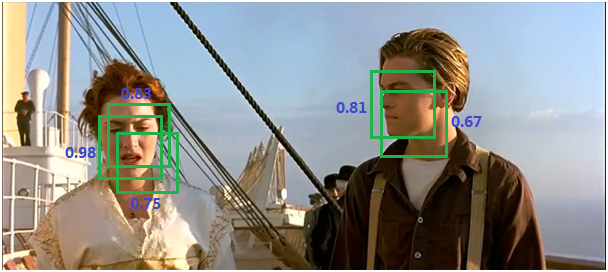
\includegraphics[scale=0.4]{nms1.png}
        \caption{Before NMS}
    \end{figure}
    
    \begin{figure}
        \centering
        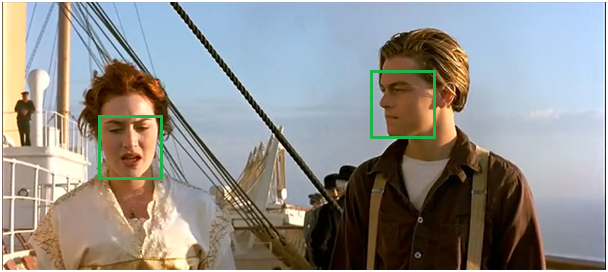
\includegraphics[scale=0.3]{nms2.png}
        \caption{After NMS}
    \end{figure}
\end{frame}

\begin{frame}{Bounding-box Regression}
    Green box: the ground truth bounding box; \\
    Red box: selective search region proposal; \\
    
    \begin{figure}
    \centering
    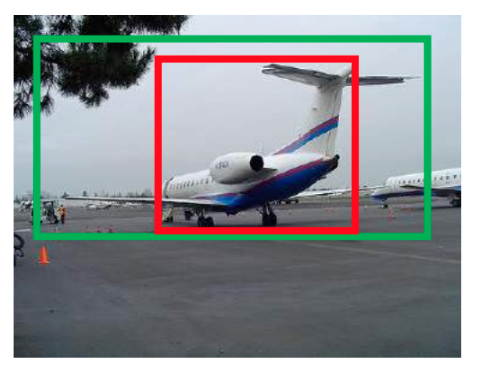
\includegraphics[scale=0.3]{img1.png}
    \end{figure}
    
    Bounding-box regression is used to adjust the red box to make it as close 
    as possible to the green one.
\end{frame}


\begin{frame}{YOLO v3 Model}
    \begin{itemize}
        \item Backbone network: Darknet-53;
        \item Anchor: total 9, but 3 for each scale;
        \item Logistic vs. Softmax: support multi-label classification;
        \item Objectness score for each box instead of each location;
    \end{itemize}
    \begin{figure}
        \centering
        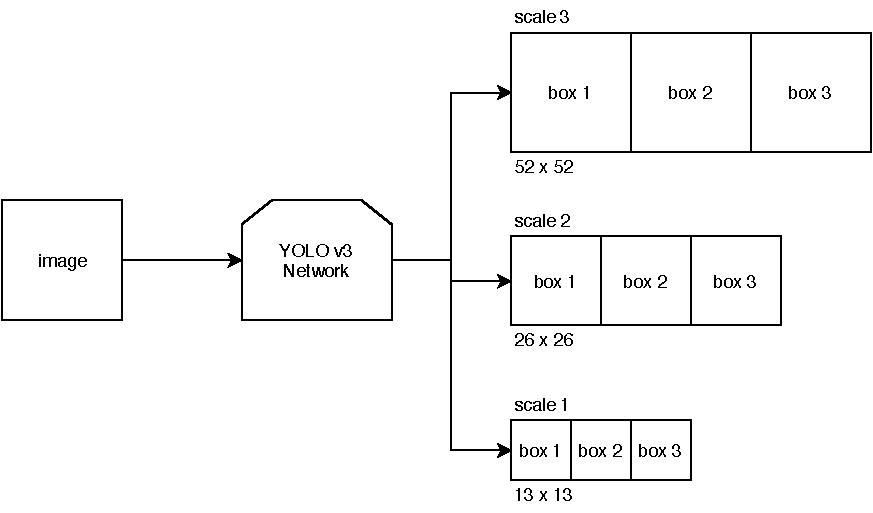
\includegraphics[scale=0.5]{yolov3_network.pdf}
        \caption{YOLO v3 process flow.}
    \end{figure}
\end{frame}

\begin{frame}{Detector Instantiation}
    \begin{figure}
        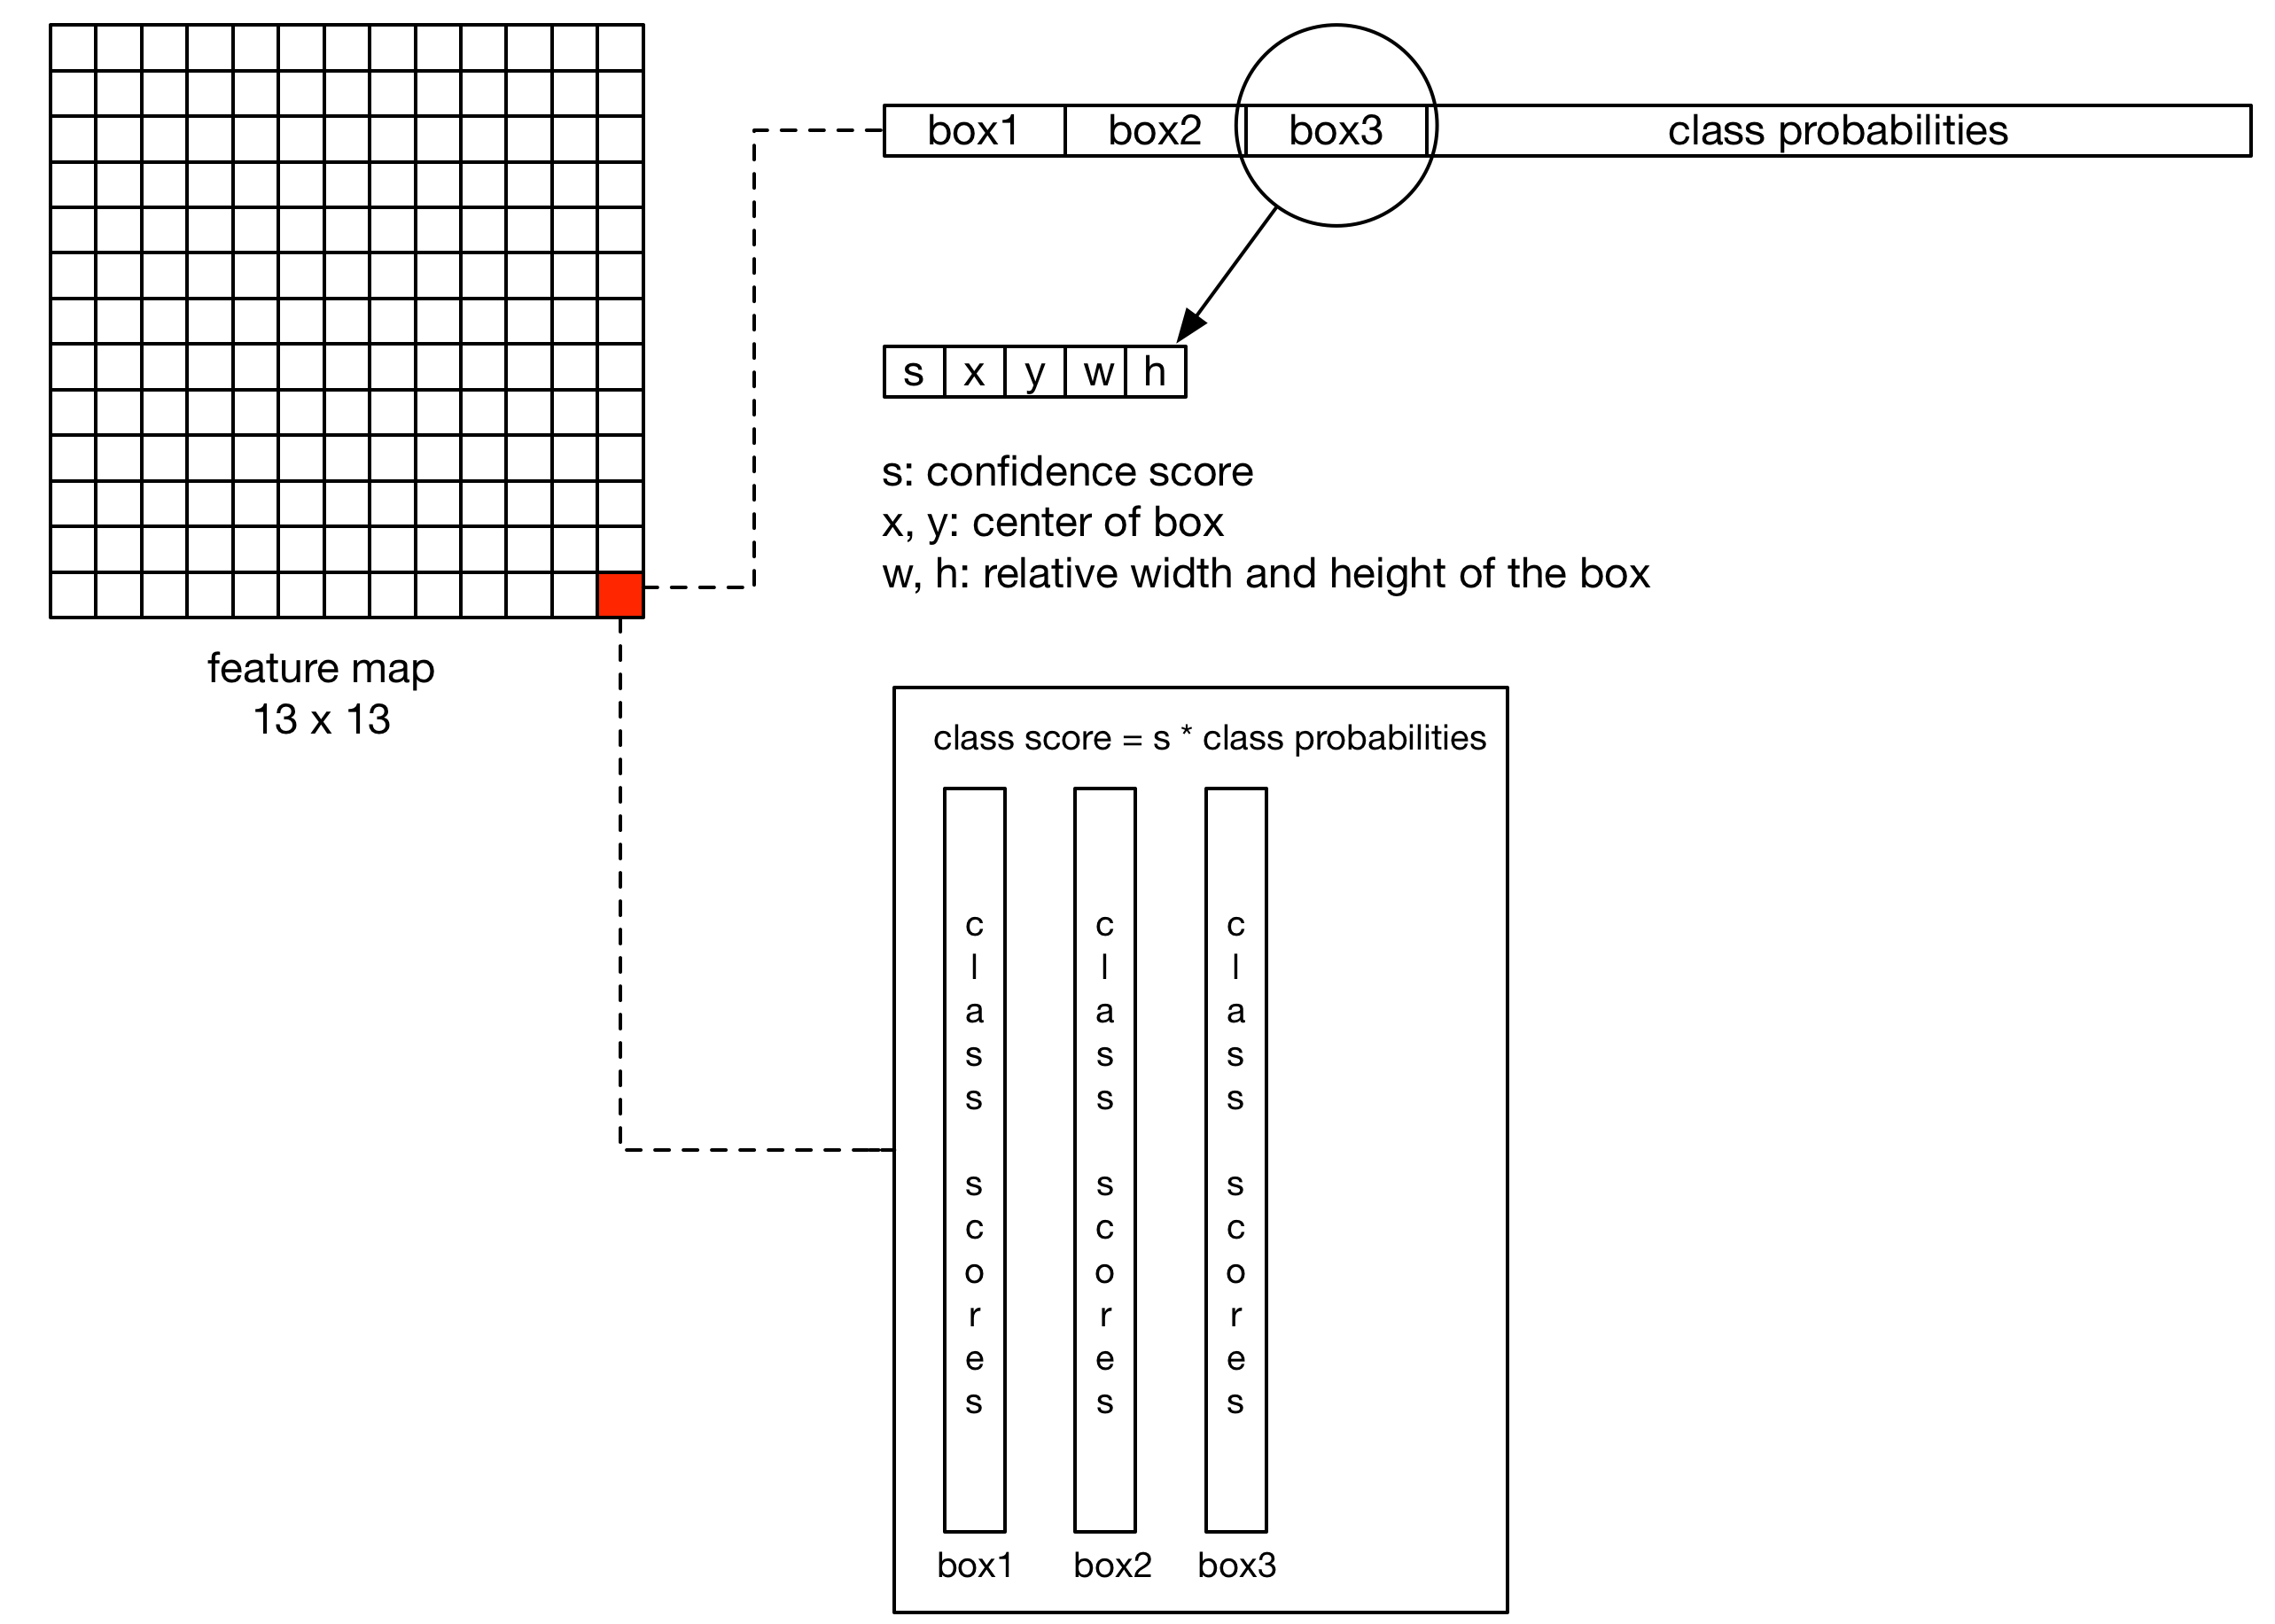
\includegraphics[width=\linewidth]{framework_detector_calc.png}
        \caption{Calculation process of each cell in the feature map.}
        \label{fig:fw-detector-calc}
    \end{figure}
\end{frame}

\begin{frame}{Detector Instantiation}
    \begin{figure}
        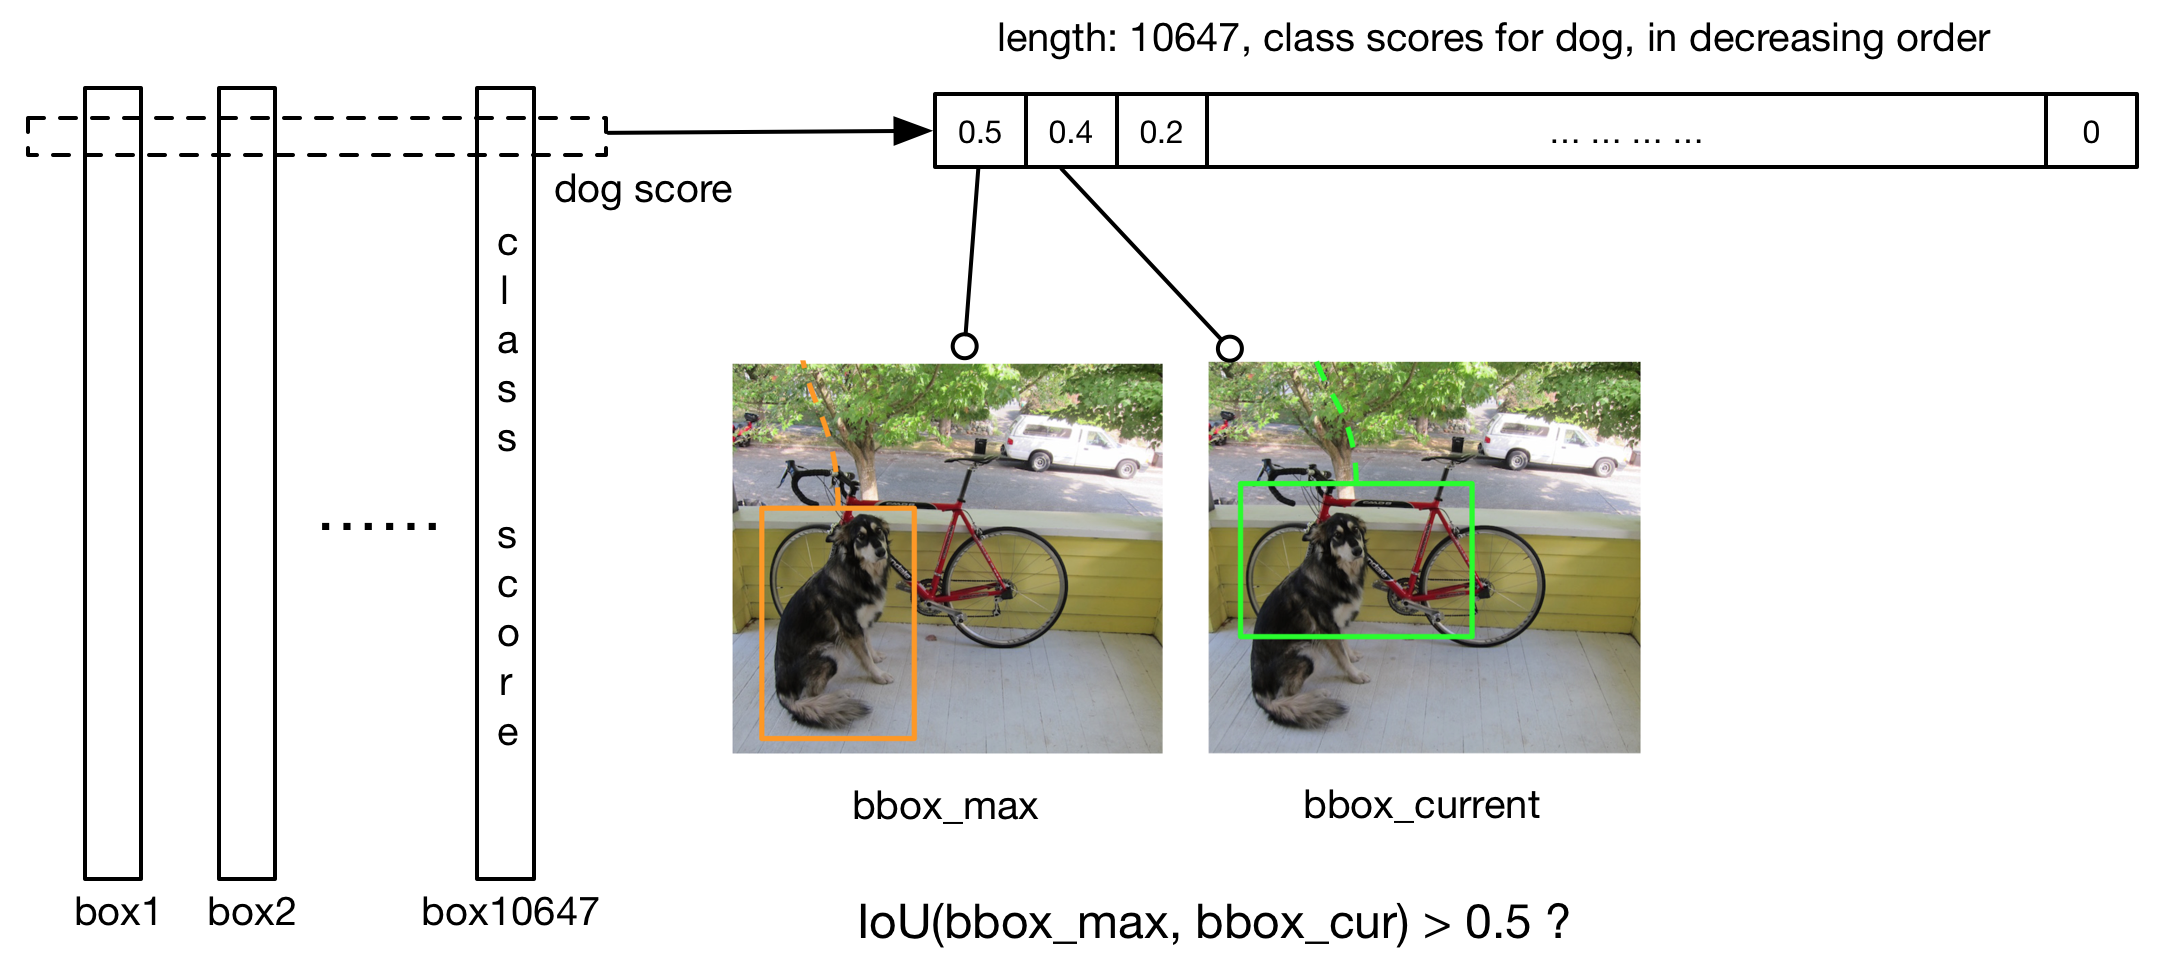
\includegraphics[width=\linewidth]{framework_detector_nms.png}
        \caption{Non-maximum suppression process.}
        \label{fig:fw-detector-nms}
    \end{figure}
\end{frame}

\begin{frame}{Person Detector Evaluation}
    \textbf{Intersection over Union Overlap}\\
    \vspace{10px}
    Intersection over Union Overlap (IoU) is used to measure how close a given 
    bounding box is to another box that is independent of the units used 
    (pixels, etc).
    \vspace{10px}
    \begin{figure}
        \centering
        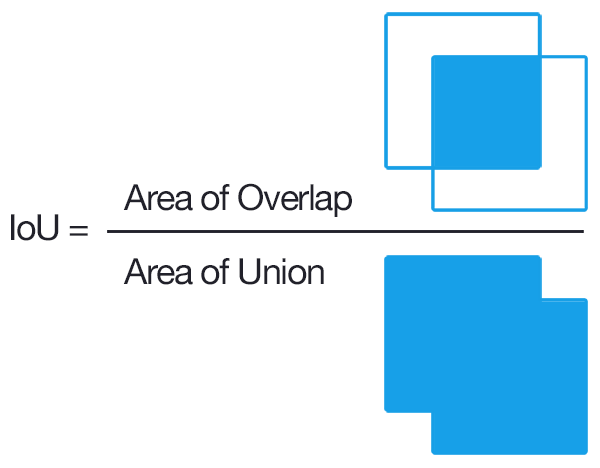
\includegraphics[scale=0.2]{iou.png} 
    \end{figure}
\end{frame}

\begin{frame}{Person Detector Evaluation}
    Possible results for one detection operation:
    \begin{itemize}
        \item True positive, a correct detection where $\mathit{IOU} \geq
        \mathit{threshold}$.
        \item False positive, a incorrect detection where $\mathit{IOU} <
        \mathit{threshold}$.
        \item True negative, does not apply.
        \item False negative, a ground truth not detected.
    \end{itemize}
\end{frame}

\begin{frame}{Person Detector Evaluation}
\textbf{Precision and Recall}\\
\vspace{5px}
\begin{description}
    \item[Precision] 
    is a fraction of relevant instances among the retrieved instances which can 
    be used to measures how accurate is your prediction.
    \item[Recall]
    is a fraction of relevant instances that have been retrieved over the total 
    amount of relevant instances. It can be used to measure how good you find 
    all the positives.
\end{description}

$$
\mathit{precision} =
\frac
{\text{\# true positive}}
{\text{\# true positive + \# false positive}}
$$

$$
\label{eq:recall}
\mathit{recall} =
\frac
{\text{\# true positive}}
{\text{\# true positive + \# false negative}}
$$
\end{frame}

\begin{frame}{Person Detector Evaluation}
    With precision and recall in hand, we can construct a Precision-Recall curve
    (P-R curve) which will be used to calculate our metric. The curve
    construction process can be described as the following:
    
    \begin{enumerate}
        \item Collect all the predictions that make for a particular class of
        objects. Rank them in decreasing order according to the confidence score
        given by the model.
        \item  Compare theses predictions with ground truth to see if they are 
        correct or not.
        \item Calculate the precision and recall using the given formula for 
        each prediction in the ranked list from top to bottom.
    \end{enumerate}
\end{frame}

\begin{frame}{Person Detector Evaluation}
    \begin{figure}
        \centering
        \begin{minipage}[b]{0.65\textwidth}
            \centering
            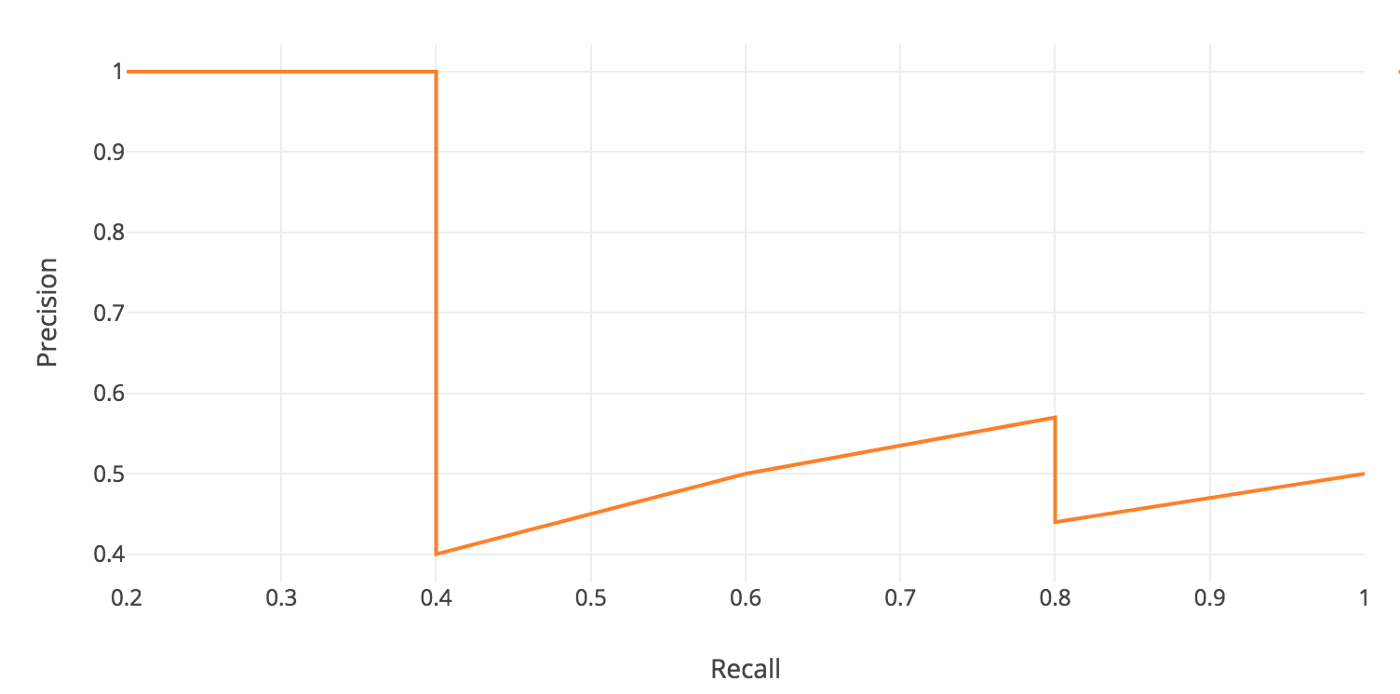
\includegraphics[width=\linewidth]{eval_pr_curve.png}
        \end{minipage}%
        \begin{minipage}[b]{0.35\textwidth}
            \centering
            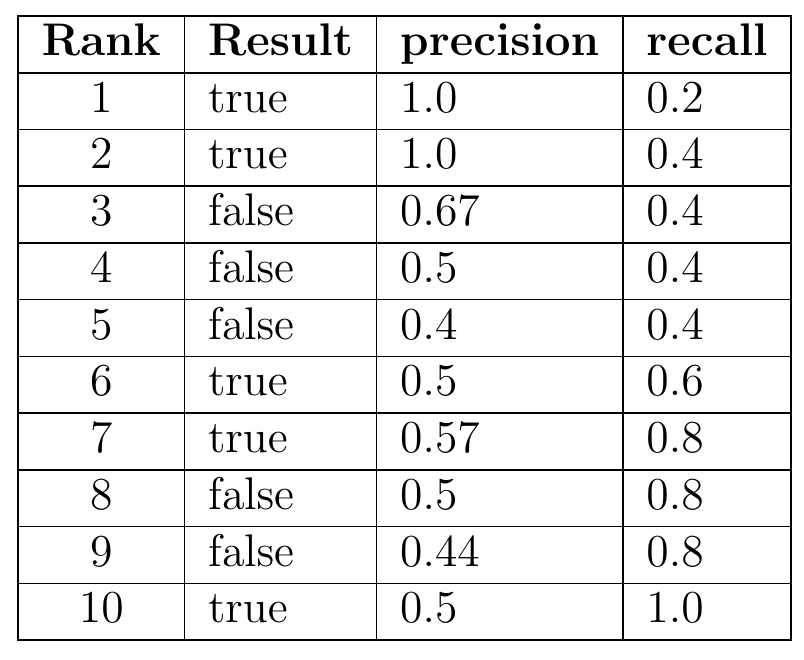
\includegraphics[width=\linewidth]{eval_pr_curve_data.png}
        \end{minipage}
        \caption[An example of Precision-Recall curve]
        {An example of P-R curve. Left is the curve itself and right is the data
            used to plot this curve, assuming that there is a total of five 
            positives
            in the data.}
        \label{fig:eval-pr-curve}
    \end{figure}
\end{frame}

\begin{frame}{Person Detector Evaluation}
    \begin{figure}
        \centering
        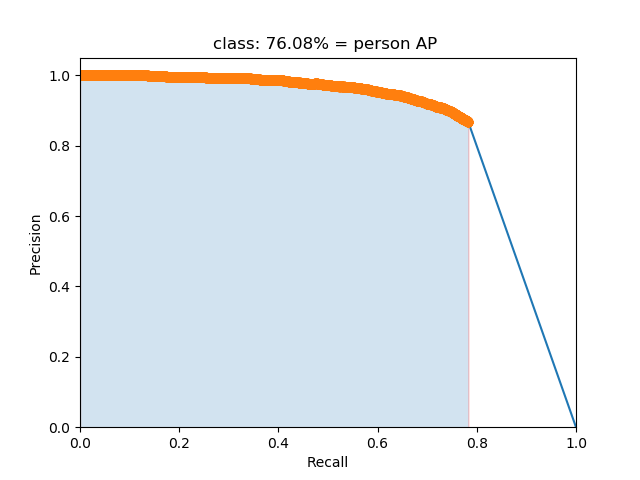
\includegraphics[scale=0.25]{eval_detector_pr_curve.png}
        \caption{Person detection model's Precision-Recall curve on 
            validation set.}
        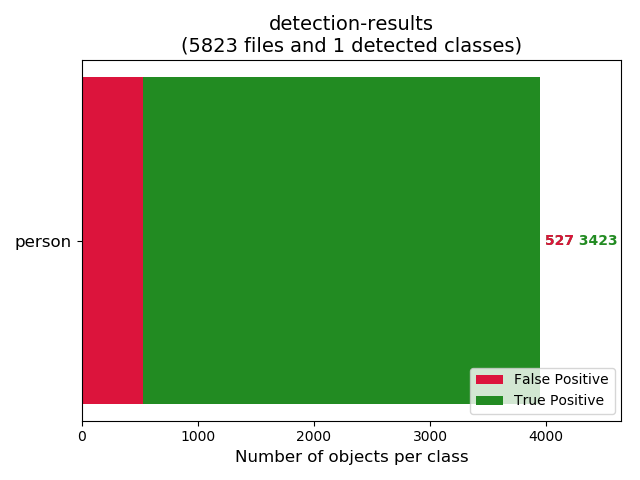
\includegraphics[scale=0.25]{eval_detector_result.png}
        \caption{Person detection result on validation set.}
    \end{figure}
\end{frame}

\begin{frame}{Person Detector Evaluation}
    \begin{figure}
    \centering
    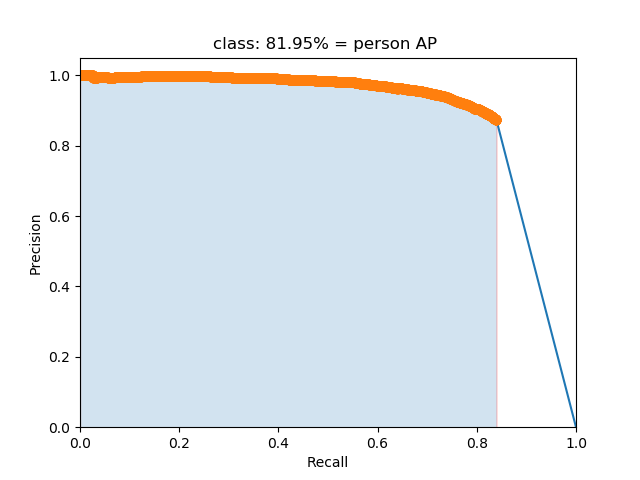
\includegraphics[scale=0.25]{eval_detector_pr_curve1.png}
    \caption{Object detection (with 20 classes supported)\\ 
        model's Precision-Recall curve on validation set.}
    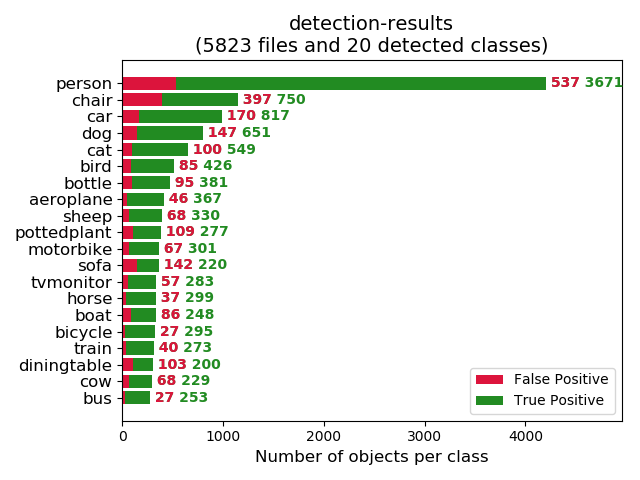
\includegraphics[scale=0.25]{eval_detector_result1.png}
    \caption{Object detection result on validation set.}
    \end{figure}
\end{frame}







\begin{frame}{Recognizer Network Architecture}
    \begin{figure}
        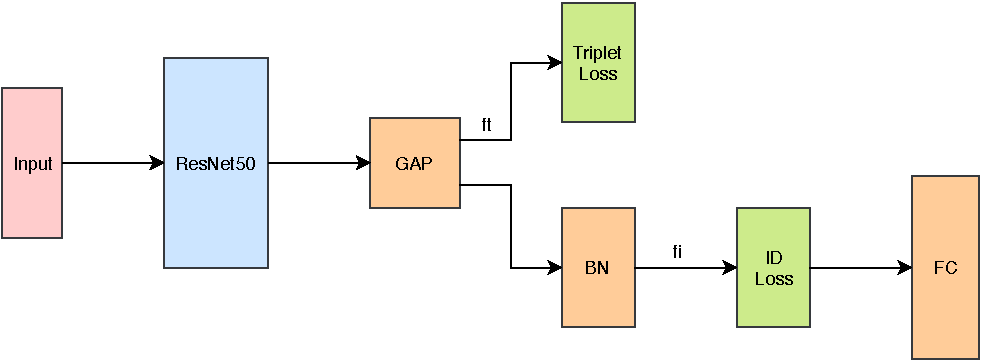
\includegraphics[width=\linewidth]{framework_reid_archit.pdf}
        \caption[Implemented recognizer network architecture]
        {
            Implemented recognizer network architecture.
                    GAP: global average pooling layer, BN: batch normalization
                    layer, FC: fully connected layer.
                    $f_t$: features used to calculate triplet loss,
                    $f_i$: features used for inference.
            The pink color represents input, blue means backbone network, 
            orange represents a special layer and green means loss function 
            layer.
        }
    \end{figure}
    \blfootnote{
        The architecture was proposed in 
        \cite{tricks-and-baseline-for-reid-2019}.}
\end{frame}


\begin{frame}{Recognizer Training Workflow}
    \begin{figure}
        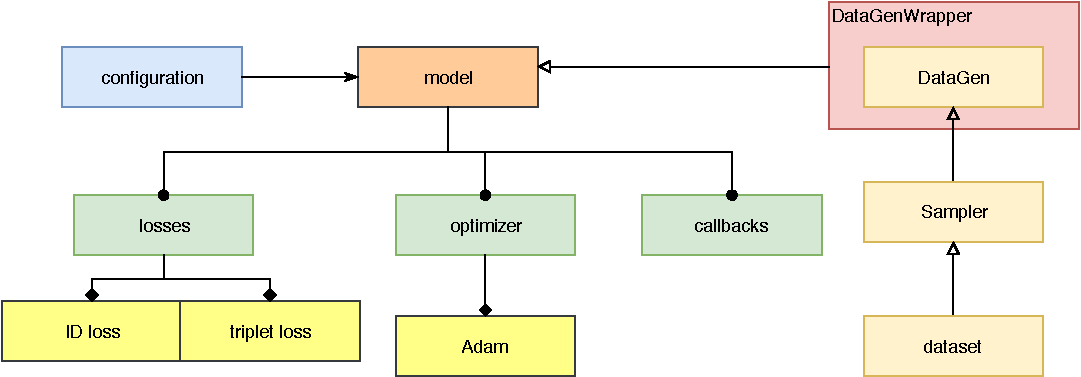
\includegraphics[width=\linewidth]{framework_reid_code_overview.pdf}
        \caption{The workflow of the ReID training program}
    \end{figure}
\end{frame}

\begin{frame}{Recognizer Training}
    \begin{itemize}
        \item batch size: $16 \times 4 = 64$
        \item warm up learning rate strategy \cite{learning-rate-warmup-2018}
        \item triplet loss + ID loss
        \item Adam optimizer
        \item total training epochs 120 \cite{tricks-and-baseline-for-reid-2019}
    \end{itemize}

    $$
        \operatorname{lr}(t)=\left\{
        \begin{array}{ll}
        {3.5 \times 10^{-5} \times \frac{t}{10}} & {\text { if } t \leq 10} \\
        {3.5 \times 10^{-4}} & {\text { if } 10<t \leq 40} \\
        {3.5 \times 10^{-5}} & {\text { if } 40<t \leq 70} \\
        {3.5 \times 10^{-6}} & {\text { if } 70<t \leq 120}
        \end{array}\right.
    $$
    
\end{frame}

\begin{frame}{Recognizer Training Visualization}
    \begin{figure}
    \begin{columns}
        \begin{column}{0.4\textwidth}
            \centering
            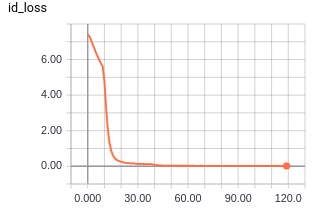
\includegraphics[width=\linewidth]{train_id_loss.png}\\
            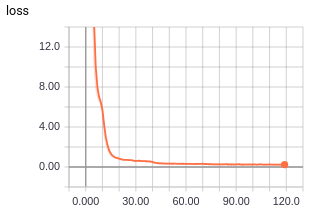
\includegraphics[width=\linewidth]{train_loss.png}
        \end{column}        
        \begin{column}{0.4\textwidth}
            \centering
            \includegraphics[width=\linewidth]{train_triplet_loss.png}\\
            \includegraphics[width=\linewidth]{train_acc.png}
        \end{column}
    \end{columns}
    \caption
    {Training visualization diagram. Upper left: training identification 
        loss curve. Upper right: training triplet hard loss curve. Lower 
        left: total training loss curve. Lower right: training 
        classification accuracy.}
    \end{figure}
    \blfootnote{These figures are produced by the TensorBoard program.}
\end{frame}














































\end{document}
